% Some general notes:
%
% - keep lines short, to improve the merge of versions

\documentclass[11pt,a4paper,twoside]{article}
\usepackage{tascar}
\usepackage{amsmath}
\usepackage[utf8]{inputenc}
\usepackage{caption}
\usepackage{subcaption}
\DeclareMathOperator*{\argmax}{arg\,max}
\DeclareMathOperator*{\argmin}{arg\,min}
\usepackage{mathtools}
\usepackage{listings}
\usepackage{framed,color}
\definecolor{shadecolor}{rgb}{1,0.9,0.8}

\definecolor{mygreen}{rgb}{0,0.6,0}
\definecolor{mygray}{rgb}{0.5,0.5,0.5}
\definecolor{mygraybg}{rgb}{0.9,0.95,0.95}
\definecolor{mymauve}{rgb}{0.58,0,0.82}
\definecolor{bole}{rgb}{0.47, 0.27, 0.23}

\newenvironment{tscattributes}
{\begin{snugshade}
\begin{tabular}{p{0.25\columnwidth}p{0.7\columnwidth}}
{\bf Attributes:}\\
\hline
}{
\hline
\end{tabular} 
\end{snugshade}
}

\newenvironment{tscelements}
{\begin{snugshade}
\begin{tabular}{p{0.97\columnwidth}}
{\bf Sub-elements:}\\
\hline
}{
\\\hline
\end{tabular} 
\end{snugshade}
}



\DeclarePairedDelimiterX{\norm}[1]{\lVert}{\rVert}{#1}

\begin{document}
\MHAtitle{User Manual}
\newpage
\tableofcontents
\newpage
\pagenumbering{arabic}

\renewcommand{\ttdefault}{pcr}

\newtcbox{\attrbox}{nobeforeafter,tcbox raise base,
arc=0pt,outer arc=0pt,colback=mygraybg,colframe=black,
boxsep=0pt,left=1pt,right=1pt,top=2pt,bottom=2pt,
boxrule=0.2pt,fontupper=\small\ttfamily}

\newtcbox{\keybbox}{nobeforeafter,tcbox raise base,
arc=2pt,outer arc=2pt,colback=mygraybg,colframe=black,
boxsep=0pt,left=1pt,right=1pt,top=2pt,bottom=2pt,
boxrule=0.2pt,fontupper=\small\ttfamily}

\newtcbox{\elembox}{nobeforeafter,tcbox raise base,
arc=0pt,outer arc=0pt,colback=mygraybg,colframe=black,colupper=h4aBlueDark,
boxsep=0pt,left=1pt,right=1pt,top=2pt,bottom=2pt,
boxrule=0.2pt,fontupper=\small\ttfamily\bfseries}

\newcommand{\refelem}[2][]{
  \ifthenelse{\equal{#1}{}}{
    \hyperref[sec:#2]{\elembox{<#2/>}}
  }{
    \hyperref[sec:#1]{\elembox{<#2/>}}
  }
  \index{#2}
}
\newcommand{\elem}[1]{\elembox{<#1/>}\index{#1}}
\newcommand{\indattr}[1]{\attrbox{\lstinline{#1}}\index{#1 (attribute)}}
\newcommand{\attr}[1]{\attrbox{\lstinline{#1}}}
\newcommand{\indmod}[1]{\hyperref[sec:#1]{{\bf #1}}\index{#1 (module)}}
\newcommand{\indapmod}[2][]{
  \ifthenelse{\equal{#1}{}}{
    \hyperref[sec:ap_#2]{{\bf #2}}\index{#2 (audio plugin)}
  }{
    \hyperref[sec:ap_#1]{{\bf #2}}\index{#2 (audio plugin)}
  }
}
\newcommand{\keyb}[1]{\keybbox{\lstinline{#1}}}

\section*{Preface}

This user manual is -- as the whole \tascar{} toolbox -- work in
progress. Bug reports and feature wishes, like, for example, improved
documentation of specific features, should directly sent to any of the
authors of \tascar{}.

\section{Introduction}

\tascar{} -- toolbox for acoustic scene creation and rendering -- is a
software designed for Linux, which allows to create virtual acoustic
environments \citep{Grimm2015a,Grimm2016a}. By means of \tascar{}, the sound
environment, which could in reality be heard in a given space and
time, can be simulated. In \tascar{} we can design virtual acoustic
environments, which we call acoustic {\em scenes} here, which are then
rendered in real time and can be played back using an arbitrary
playback system. These virtual acoustic scenes made using \tascar{}
can also be interactively explored by the user in the real time for
example using headphones and a joy-stick to steer the movement in
acoustic space.

However, it should be noted, that \tascar{} is not a room acoustics
simulator and the goal of \tascar{} is not to exactly reproduce the sound
field in a room, but to provide a fast and perceptively plausible
method for rendering virtual acoustic environments in real time. The
\tascar{} software is principally suited for building dynamic and
interactive environments, which can be applied in hearing aid
development and evaluation, psycho-physics with adaptive changes of
the spatial configuration, soundscape simulations and computer
games. There is almost unlimited variety of the environments, which
can be simulated using \tascar{} and a user has an opportunity to specify
the content and dynamics of an acoustic scene very precisely.

An acoustic scene in its simplest form consists of three types of
objects: sound sources, receiver and reflectors.  
%
Each object has a position and orientation in the virtual space in a
given time.
%
To simulate an object in motion, the object's position or orientation
have to change over time.

The position of the receiver corresponds to the point in the virtual
space for which the simulation is currently being done, while the
receiver's orientation influences the received sound, based on
effective relative direction of arrival, if the used receiver type is
not omni-directional.
%
To simulate the sound that would be audible at the receiver's position
at some point in time, some signal processing has to be performed,
mimicking acoustic phenomena like reflection, air absorption or
diffraction.
%
These acoustic simulation methods will be discussed in detail in the
second chapter.

A list of \tascar{}-rendered scenes is described in
\citet{Grimm2016}. Validation of the principle applicability to
hearing aid research can be found in \citet{Grimm2015b}. Distance
perception was evaluated in \citet{Grimm2015c}.


\section{General remarks and invocation}

\tascar{} is provided as a Debian package. You will receive
information on how to set up the software package system to include
the \tascar{} package repository from your project partner.  Table
\ref{tab:instdir} provides a list of installation directories.

\begin{table}[htb]
\hrule
\medskip
\begin{tabular}{ll}
\verb!/usr/share/doc/tascar!      & documentation and user manual   \\
\verb!/usr/share/tascar/examples! & example files                   \\
\verb!/usr/share/tascar/matlab!   & tools for MATLAB and GNU Octave \\
\verb!/usr/share/tascar/python!   & tools for python/blender        \\
\end{tabular}
\medskip
\hrule
\caption{List of relevant \tascar{} directories\index{directories}.}\label{tab:instdir}
\end{table}

After successful installation of the packages,
\tascar{} is available as the command \verb!tascar! or from the main
applications menu, in the ``sounds and video'' section.

\tascar{} is heavily relying on the jack audio connection kit
(\url{http://jackaudio.org}). It is required to start jack before
loading a session into \tascar{}. Jack port names in \tascar{} are
treated as POSIX regular expressions \cite{posixregexp}. If the
\verb!^! or \verb!$! anchors are not present at the beginning or end
of an expression, they are added at beginning and end of expression to
achieve proper full name matching. Please note that some characters
like \verb!.[?()! (and some more) have special meaning as regular
expression and need to be quoted for correct matching.

An acoustic environment can be loaded using either the command line by
providing the file name, or via the file menu in the main window. If
loading of a session file fails for some reason, it might be helpful
to start it at the command line to see additional information.

\tascar{} uses SI units unless specified otherwise. Developers of new
plugins are encouraged to use SI units for all internal and
configuration variables.

\subsection{Keyboard shortcuts in the main window}

The \tascar{} GUI can be controlled using keyboard shortcuts.

\parbox{\columnwidth}{ 

Changing the view in the main window between
the elements of the menu bar on the left side:

\begin{tabular}{|ll|}
  \hline
\keyb{Alt}+\keyb{1} & Map           \\
\keyb{Alt}+\keyb{2} & Mixer         \\
\keyb{Alt}+\keyb{3} & XML source    \\
\keyb{Alt}+\keyb{4} & OSC variables \\
\keyb{Alt}+\keyb{5} & Licenses      \\
\keyb{Alt}+\keyb{6} & Warnings     \\
\keyb{Alt}+\keyb{7} & News     \\
\hline
\end{tabular}

}

\parbox{\columnwidth}{ 

Opening the top menu bar elements:

\begin{tabular}{|ll|}
  \hline
\keyb{Alt}+\keyb{F} & File      \\
\keyb{Alt}+\keyb{T} & Transport \\
\keyb{Alt}+\keyb{V} & View      \\
\keyb{Alt}+\keyb{H} & Help     \\
\hline
\end{tabular}
}

\parbox{\columnwidth}{ 

Opening and closing \tascar{} files:

\begin{tabular}{|ll|}
  \hline
\keyb{Ctrl}+\keyb{N} & Open new \tascar{} scene       \\
\keyb{Ctrl}+\keyb{O} & Open a \tascar{} file          \\
\keyb{Ctrl}+\keyb{X} & Open an example \tascar{} file \\
\keyb{Ctrl}+\keyb{R} & Revert to previous scene       \\
\keyb{Ctrl}+\keyb{W} & Close \tascar{} scene          \\
\keyb{Ctrl}+\keyb{Q} & Quit the program               \\
\hline
\end{tabular}

}

\parbox{\columnwidth}{ 

Controlling the transport of a \tascar{} scene:

\begin{tabular}{|ll|}
  \hline
\keyb{Space}        & Play                             \\
\keyb{Ctrl}+\keyb{Space} & Stop                             \\
\keyb{Page Up}      & Rewind                           \\
\keyb{Page Down}    & Forward                          \\
\keyb{Home}         & Previous                         \\
\keyb{End}          & Next                             \\
  \hline
\end{tabular}

}

To show more information about an element of the scene, it can be
selected in the Map view (Alt 1) by clicking on the origin of the object. The
gain controller and the corresponding part of the XML source code will
be displayed on the right side of the window, allowing to switch
between the elements by using the drop-down menu in the top right
corner. There is also an option to track the selected object.


\subsection{Optimization of the operating system for audio processing}

Configure real-time scheduling: grant permissions to aquire real-time
priority, and to lock memory in RAM, to users in group 'audio' (edit
{\tt /etc/security/limits.conf}):

\begin{verbatim}
@audio - rtprio	 99
@audio - memlock unlimited
\end{verbatim}

Add desired user of tascar (in this example, this user is named 'tascar')
to group 'audio':
\begin{verbatim}
adduser tascar audio
\end{verbatim}
Log out and log in again (no re-boot required).

Deactivate CPU frequency scaling in BIOS, or switch to maximum
performance manually, e.\,g., with
\begin{verbatim}
for c in {0..11}; do cpufreq-selector -c $c -g performance; done
\end{verbatim}
or with the \tascar{} provided wrapper \verb!tascar_cpufreq!.

\subsection{Overwriting application default values}\label{sec:globalconfig}

Some variables which are not session related have built-in default
values. These values can be overwritten using an external application
configuration file in XML format. The files
\verb!/etc/tascar/defaults.xml! and \verb!${HOME}/.tascardefaults.xml!
  are read in this order, i.e., values in the second file overwrite
  the system defaults. To see the configurable variables, set the
  environment variable \verb!TASCARSHOWGLOBAL! to ``yes'' start the
  application from the command line, e.g.,
\begin{verbatim}
TASCARSHOWGLOBAL=yes tascar
\end{verbatim}
or
\begin{verbatim}
TASCARSHOWGLOBAL=yes tascar_spkcalib
\end{verbatim}
%
An example application configuration file can look like this:
\begin{verbatim}
<tascar>
  <spkcalib>
    <inputport data="system:capture_29"/>
    <reflevel data="80"/>
  </spkcalib>
</tascar>
\end{verbatim}
%
This will translate into these variables:
\begin{verbatim}
tascar.spkcalib.inputport (system:capture_29)
tascar.spkcalib.reflevel (80)
\end{verbatim}

\section{Scene Definition}

Acoustic scenes are created using xml scene definition file
format\index{file format}. \tascar{} scene definition (\verb!.tsc!-file) is a text xml
file, where the user specifies all the details about the scene using
various commands (elements and their attributes). An example of a
scene definition is shown below (example file \verb!example_basic.tsc!):
\tscexample{example_basic}

\refelem{scene}, \refelem{receiver}, \refelem{face},
\refelem{source} etc.\ are the elements and \textbf{name},
\textbf{loop}, \textbf{reflectivity}, \textbf{width} etc.\ are their
attributes. Figure \ref{fig:tascar_scene_example} shows the
representation of this scene definition in \tascar{}.
%
The main window\index{main window} contains a toolbar for file
interactions, transport and time control, and controls for muting and
soloing the different components of the scene (left panel).
%
The scene map window contains a visual representation of the
scene. Editing the scene via the graphical user interface is currently
not possible.

\begin{figure}[htb]
    \centering
    \fbox{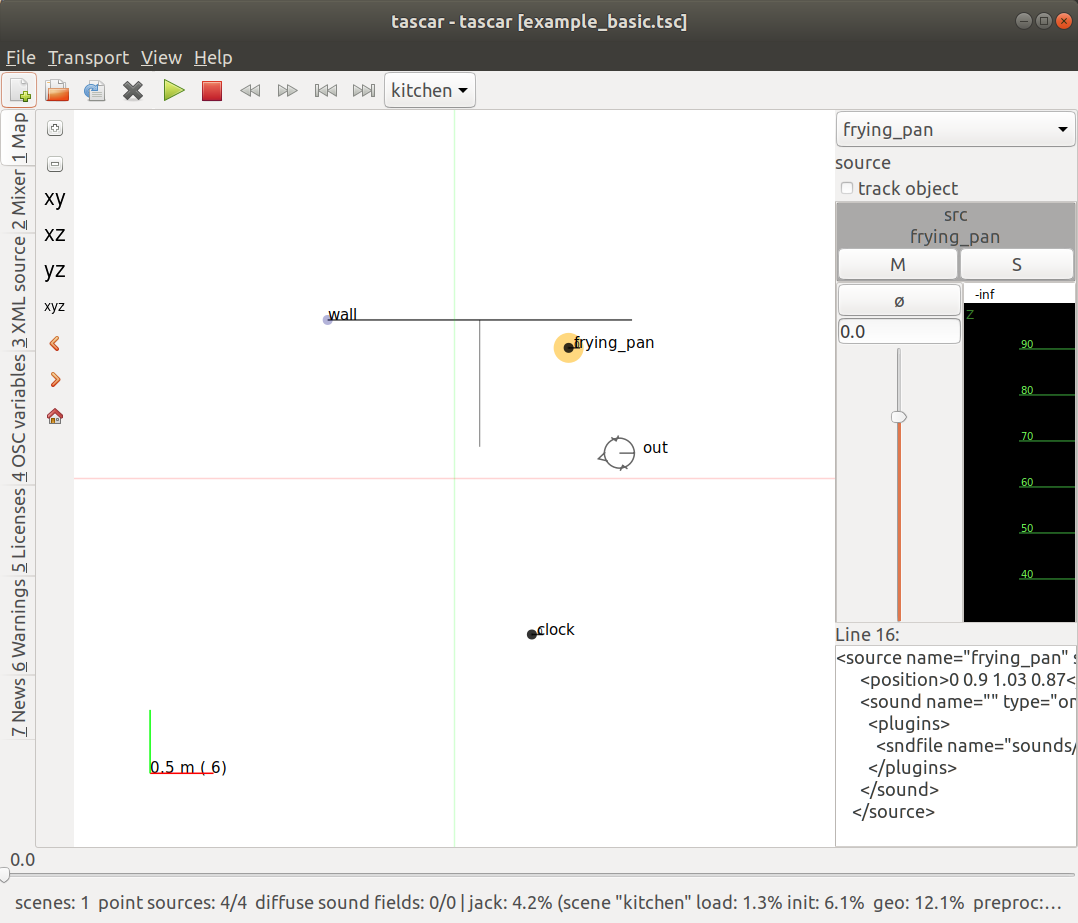
\includegraphics[width=\textwidth]{tascarpro_mainwindow.png}}
    \caption{Simple \tascar{} scene example. Scene consist of two sources, one reflector and one receiver. }
    \label{fig:tascar_scene_example}
\end{figure}

%\framebox[1.1\width]{\textbf{tascar example\_ktchen.tsc}} \\

Note: In general, if an attribute or a element is not specified in
the scene definition, it is set to default. Therefore, it is not
necessary to specify all the recognized attributes and elements.

\section{Top level elements}

Elements \refelem{session} and \refelem{scene} are referred to as
top-level elements in \tascar{} documentation.
%
One \refelem{session} element can contain multiple \refelem{scene}
elements.
%
Together, they form the outermost building blocks of \tascar{} scenes.

\subsection{The {\tt <session>...</session>} element}\label{sec:session}\index{session}

\elem{session} is the root element of each scene definition file. It
can contain one or more scenes (\refelem{scene}), port connections
(\refelem{connection}), external modules (\refelem{modules}) and range
definitions (\refelem{range}).

\begin{tscattributes}
\indattr{name}               & Name of session (default: ``tascar'')                                                \\
\indattr{duration}           & Duration of session in seconds; default: 60                                          \\
\indattr{loop}               & Loop session (true|false); default: false                                            \\
\indattr{levelmeter\_tc}     & Level meter time constant in seconds; default: 2                                     \\
\indattr{levelmeter\_weight} & Level meter weight type; default: Z (currently the only one)                         \\
\indattr{levelmeter\_min}    & Level meter minimum in dB (default: 30)                                              \\
\indattr{levelmeter\_range}  & Level range of level meters in dB (default: 70)                                      \\
\indattr{levelmeter\_mode}   & Level meter mode (rms, rmspeak, percentile)                                          \\
\indattr{srv\_addr}          & OSC server multicast address, empty uses unicast                                     \\
\indattr{srv\_port}          & OSC server port number (default: 9877), or ``none'' to deactivate OSC server         \\
\indattr{warnsrate}          & Print a warning if the system sampling rate doesn't match the specified one          \\
\indattr{requiresrate}       & Stop loading the session if the system sampling rate doesn't match the specified one \\
\indattr{warnfragsize}       & Print a warning if the system fragment size doesn't match the specified one          \\
\indattr{requirefragsize}    & Stop loading the session if the system fragment size doesn't match the specified one \\
\indattr{license}            & License form of session file                                                         \\
\indattr{attribution}        & Attribution of session file, e.g., author name                                       \\
\end{tscattributes}

A session can have sub-elements \elem{mainwindow} and \elem{mapwindow}
to control the window positions. These attributes are allowed:
\begin{tscattributes}
\indattr{x}     & x-position of window                                         \\
\indattr{y}     & y-position of window                                         \\
\indattr{w}     & Width of window (default: 1600)                                         \\
\indattr{h}    & Height of window (default: 480)                                         \\
\end{tscattributes}

An example of a session with multiple scenes is:
\tscexample{example_multiplescenes}

The jack transport can be controlled via the OSC paths {\tt
  /transport/start}, {\tt /transport/stop} and {\tt
  /transport/locate}.

A special sub-element \refelem{include} can be used to include scenes
and other elements from another session file, given by the attribute
\indattr{name}. Example:
\begin{lstlisting}[numbers=none]
<?xml version="1.0"?>
<session>
  <include name="session1.tsc"/>
  <include name="session2.tsc"/>
</session>
\end{lstlisting}
\begin{tscattributes}
\indattr{name}        & File name to be included                       \\
\indattr{license}     & License form of session file                   \\
\indattr{attribution} & Attribution of session file, e.g., author name \\
\end{tscattributes}

The \refelem{include} element can also be used at other levels; the
only limitation is that the root element of the included file needs to
match the active element into which the external file is included.
%
In the example given above, the root XML element of files
{\verb!session1.tsc!} and {\verb!session2.tsc!} has to be a
\refelem{session} element.
%
Any attributes given to the root element of the included file that
differ from the attributes of the same element in the including file
are ignored.
% Comment: This is counter-intuitive.  It is probably a hack to allow
% included files to allow multiple scenes (XML permits only a single
% root element).

The file names given in the name attribute of the \refelem{include}
element can be absolute or relative.
%
Relative file names are relative to the directory containing the root
\verb!.tsc!-file.
% Comment: This is achieved by changing the current working directory
% (CWD) of the tascar process before loading a .tsc file using the
% gui.  Tobias considers this to be a bug.  Relative paths should
% either be relative to the unaltered CWD of the tascar process as on
% startup, or they should be relative to the file containing the
% respective <include> element.

\subsection{The {\tt <scene>...</scene>} element}\label{sec:scene}\index{scene}

\begin{tscattributes}
\indattr{name}        & Name of scene (default: ``scene'')                        \\
\indattr{guiscale}    & Display scaling in meter; default: 200                    \\
\indattr{guicenter}   & Display center (x, y, z) in meter; default: 0 0 0         \\
\indattr{guitracking} & Track an object in the scene map (default: use guicenter) \\
\indattr{ismorder}    & Order of image source model (default: 1)                  \\
\indattr{c}           & Speed of sound in m/s; default: 340                       \\
\end{tscattributes}

\begin{tscelements}
\refelem{source}, \refelem{receiver},
\refelem{diffuse}, \refelem{face}, \refelem{facegroup},
\refelem{obstacle}, \refelem{description}
\end{tscelements}

\elem{scene} is a top-level element of a \tascar{} scene
definition. An example scene definition is given in Example
\ref{tsc:example_basic}.

\section{Objects}

A scene can be complemented with objects\index{object} of different types (as it was
already shown in the first example of a scene definition). 
%
Objects can be any of the following types:
\begin{itemize}
\item sources (\refelem{source}), diffuse sound fields (\refelem{diffuse})
\item receivers (\refelem{receiver})
\item reflectors (\refelem{facegroup}, \refelem{face})
\item obstacles (\refelem{obstacle})
\item masks (\refelem{mask})
\end{itemize}
There can be many objects of different types in the scene. Each object
has position and orientation in space and time, and may also contain
different attributes depending on the type.

There are two different ways of defining the position and orientation
of an object - ``interactive'' and ``not interactive''.
%
First, we have to specify the ``not interactive'' position and
orientation (it can be also the whole trajectory of an object) in a
scene definition file.
%
 
As an addition to this predefined geometry, we can steer the object
using an external device, for example a joystick, head movement
tracking system or by an algorithm which generates a certain type of
movement, thus applying ``interactive'' type of geometry.
%
The resulting position and orientation of an object will be calculated
by summing up these two mentioned types of position and
orientation. 
%
The difference between two types of defining the movement has been
depicted in Figure \ref{fig:positions}. 

\begin{figure}[htb]
  \centering
  \fbox{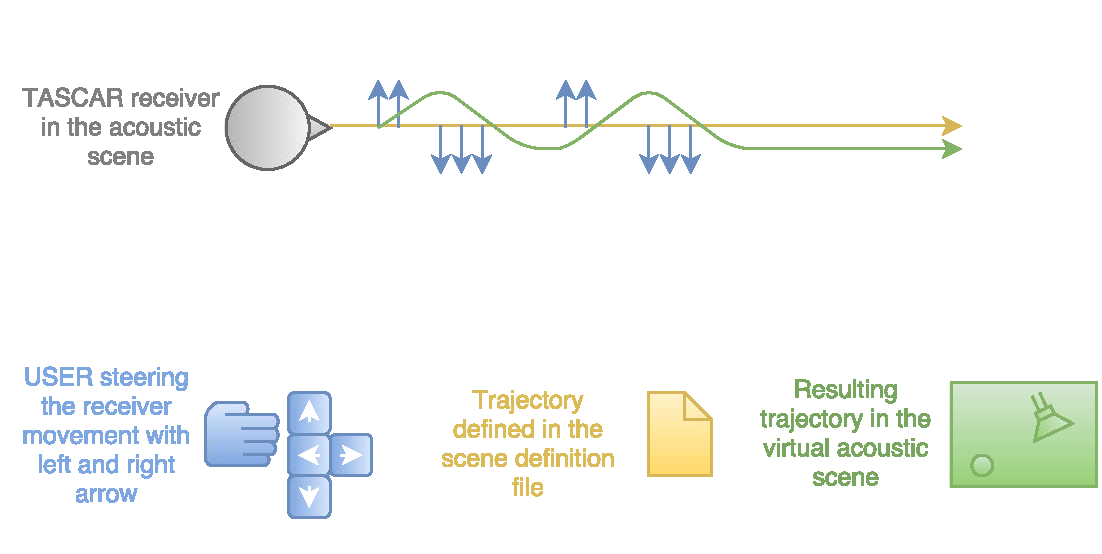
\includegraphics[width=0.8\textwidth]{positions}}
  \caption{Two different ways of dealing with orientation and position in \tascar{}
}
  \label{fig:positions}
\end{figure}



\subsection{Common attributes of objects}
\label{common attributes}

The following attributes are common to all scene objects:

\begin{tscattributes}
\indattr{name}               & Name of the object (default: "in" for {\tt source}, "out" for {\tt receiver})                                                         \\
\indattr{mute}               & Mute the object; {\tt mute="true"} or {\tt mute="false"}; default: "false"                                                            \\
\indattr{solo}               & Solo the object (i.\,e.\ mute all objects which don't have solo activated); {\tt solo="true"} or {\tt solo="false"}; default: "false" \\
\indattr{color}              & Color of the graphical representation of the object (hex triplet)                                                                     \\
\indattr{start}              & Render activity start time in seconds; default: 0                                                                                     \\
\indattr{end}                & Render activity start time in seconds; default: 0                                                                                     \\
\indattr{sampledorientation} & Sample orientation along trajectory with this distance (default: 0)                                                                   \\
\end{tscattributes}

The render activity is limited to the interval [start,end] only if end
\(>\) start. All time information of objects, such as dynamic geometry
or sound file positions, are relative to the object start time.
%
This {\em object time} is defined as session time minus object start time.

Muting an object disables it, i.\,e., muting a \verb!source! will
disable the sound, muting a \verb!receiver! will disable the output of
the receiver, and muting a \verb!face! or \verb!facegroup! will
disable all image sources generated by that reflector.


\subsection{Common sub-elements of objects}

All scene objects (e.g. instances of
\refelem{source}, \refelem{receiver}, \refelem{mask},
\refelem{facegroup}, \refelem{face}, etc.) have to define their
position and orientation in space and time.
%
The following child elements can be used to specify these parameters
(see also Example \ref{tsc:example_basic}).
 
\subsubsection{The {\tt <position>...</position>} element}\label{sec:position}\index{position}

Position is specified by providing Cartesian coordinates (in meters)
as well as the time point associated with them (object time in
seconds, counted with respect to the time when the object starts to be
active, see attribute \attr{start} of parent element):
\itscexamplepriv[linerange={1-1},numbers=none]{pos_and_rot}

If we want the object to change its position over the course of the
scene, we have to specify more than one point in space and time:
%
\itscexamplepriv[linerange={3-7},numbers=none]{pos_and_rot}
t\_n is time and x\_n, y\_n and z\_n are the Cartesian coordinates of
an object at time t\_n.  The object's position will be linearly
interpolated between these points.
%
The numbers are separated by white space.
%
The line breaks in this example are solely for human readability,
and not required by the \tascar{} software.

We can also use an attribute to control the interpolation method:
\itscexamplepriv[linerange={9-16},numbers=none]{pos_and_rot}
The first example will interpolate linearly in Cartesian coordinates,
i.\,e., the object will move on a straight line from (1,4,0) to
(1,-4,0). 
%
The second example will interpolate linearly in spherical coordinates
around the origin, i.\,e., the object will move along an arc from
(1,4,0) to (1,-4,0).

The last position of the position track is held until the either the
session, or the current position loop iteration (see below),
terminates.

Instead of defining the position track in the tsc file it can also be
read from a comma-separated file, by setting the attribute
\indattr{importcsv}.

Position tracks and orientation tracks can be looped by adding the
attribute \indattr{loop} with a number larger than zero.

\begin{lstlisting}[numbers=none]
  <position loop="10">0 0 0 0
  6 10 0 0</position>
\end{lstlisting}

in this case, the position/orientation is sampled with the object time
modulo loop time (10 seconds), i.\,e., the object is moving for 6
seconds, then resting at (10,0,0) for 4 seconds, then again moving for
6 seconds, starting at (0,0,0).

\begin{tscattributes}
  \indattr{interpolation}
  &
  Coordinate system in which positions are linearly interpolated
  between given positions. Possible values are {\tt cartesian} and
  {\tt spherical}. Default: {\tt cartesian}.
  \\
  \indattr{importcsv}
  &
  Read position track from the given \verb!.csv!-file as
  comma-separated values.  The given file name can contain absolute or
  relative path.  Relative paths are relative to the session's
  \verb!.tsc!-file. Default: position track is contained as
  space-separated text between opening and closing \refelem{position}
  tags.
  \\
  \indattr{loop}
  &
  The value, if greater than {\tt 0}, specifies the time in seconds
  when this position track is repeated from {\tt 0}. Default: {\tt 0},
  no repetition.
  \\
\end{tscattributes}

\subsubsection{The {\tt <orientation>...</orientation>} element}\label{sec:orientation}\index{orientation}

Orientation is specified in Euler (navigation) angles $R_{z,y,x}$, measured in degrees:
%
\itscexamplepriv[linerange={18-18},numbers=none]{pos_and_rot}
$R_z$ is the rotation around the z-axis, $R_y$ around the y-axis and
$R_x$ around the x-axis. They are applied in z,y,x order, after
application of the position.
%
If we would like the orientation of an object to change during the
scene, we can specify multiple angles and time points associated with
them:
\itscexamplepriv[linerange={20-23},numbers=none]{pos_and_rot}
%
The numbers are separated by white space.
%
The line breaks in this example are solely for human readability,
and not required by the \tascar{} software.

The last orientation of the orientation track is held until the either
the session, or the current orientation loop iteration (see below),
terminates.

Instead of defining the orientation directly in the tsc file it can
also be read from a comma-separated file, by setting the attribute
\indattr{importcsv}.

Euler orientation tracks can be looped by adding the attribute
\indattr{loop} with a number larger than zero.

\begin{tscattributes}
  \indattr{importcsv}
  &
  Read orientation track from the given \verb!.csv!-file as
  comma-separated values.  The given file name can contain absolute or
  relative path.  Relative paths are relative to the session's
  \verb!.tsc!-file. Default: orientation track is contained as
  space-separated text between opening and closing
  \refelem{orientation} tags.
  \\
  \indattr{loop}
  &
  The value, if greater than {\tt 0}, specifies the time in seconds
  when this orientation track is repeated from {\tt 0}. Default:
  {\tt 0}, no repetition.
  \\
\end{tscattributes}

\subsubsection{The {\tt <creator>...</creator>} element}\label{sec:creator}\index{creator}

Instead of defining the object's movement manually (defining position
and orientation for each time point) we can use the creator tool.
\tscexamplepriv[linerange={8-14},firstnumber=8]{example_cashdesk} In
this case, the orientation is calculated as a tangent along the given
path.

\subsubsection{Delta-transformations}\label{sec:deltatransform}\index{delta-transformation}

In addition to the transformation defined by the \elem{position},
\elem{orientation} and \elem{creator} elements, every object has a
delta-transformation which can be controlled via OSC or by actor
modules (see section \ref{sec:actormod}).

\subsubsection{The {\tt <navmesh/>} element}\label{sec:navmesh}\index{navmesh}\index{navigation mesh}

The navmesh element can be used to restrict the object motion to a
navigation mesh.
%
This is specifically useful when controlling object positions via game
controllers.

\begin{tscattributes}
\indattr{importraw} & File name of raw file containing list of polygon surfaces. \\ 
\indattr{maxstep}   & Maximal vertical step size.                                \\ 
\indattr{zshift}    & Vertical shift of control position, to achieve 
above-floor positions with a floor navigation mesh.                              \\
\end{tscattributes}

Faces can be imported from a text file, containing space-separated
lists of polygon coordinates (see section \ref{sec:facegroup} on face
groups for details), or within the \elem{faces} sub-element.

\subsection{The {\tt <source>...</source>} element}\label{sec:source}\index{source}

\underline{Recognized attributes:}

\refelem{source} supports the attributes common to
all scene objects, refer to section \ref{common attributes}
\nameref{common attributes} on page \pageref{common attributes} for
details.

\underline{Recognized sub-elements:} 

\refelem{position}, \refelem{orientation}, \refelem{creator}, \refelem{sound}

\elem{source} is an element used to create the sound source
objects in the scene definition. Since sources are also objects, they
have to have a certain position and orientation in space.  A source
object can consist of one or more "sound vertices" specified with a
sub-element \refelem{sound}. There must also be a sound content, for
example from a sound file, assigned to a source. We can assign a sound
content to a source using the audio plugin
\refelem[ap_sndfile]{sndfile}.

In the box below we can see a definition of a simple point source
object (taken from Example \ref{tsc:example_basic}):
\tscexamplepriv[linerange={16-23},firstnumber=16]{example_basic}

\subsubsection{The {\tt <sound .../>} element}\label{sec:sound}\index{sound}\index{vertex}

\begin{tscattributes}
\indattr{type}                       & Sound source radiation type (default: ``omni'')                                            \\
\indattr{gainmodel}                  & Gain model, either ``1/r'' or ``1'' (default: ``1/r'')                                     \\
\indattr{size}                       & Physical size for source width simulation\footnote{Currently only used by receiver hoa2d.} \\
\indattr{sincorder}                  & Sinc interpolation order, 0 = nearest neighbor; default: 0                                 \\
\indattr{caliblevel}                 & Calibration level in dB; default: 93.9794                                                  \\
\indattr{gain}                       & Gain in dB; default: 0                                                                     \\
\indattr{x},\indattr{y}, \indattr{z} & Local Cartesian coordinates; default: 0                                                    \\
\indattr{d}                          & Chain distance (vertex distance along trajectory); default: 0                              \\
\indattr{maxdist}                    & Maximum delay line length in meter; default: 3700                                          \\
\indattr{minlevel}                   & Minimum SPL for source to be rendered (default: -inf)                                      \\
\indattr{ismmin}                     & Minimal ISM order to be rendered (0)                                                       \\
\indattr{ismmax}                     & Maximal ISM order to be rendered ($2^{32}$)                                                \\
\indattr{layers}                     & List of active layers, or empty for all layers (default)                                   \\
\indattr{airabsorption}              & Render air absorption (default: true)                                                      \\
\indattr{name}                       & Name (postfix)                                                                             \\
\indattr{connect}                    & Jack port connection                                                                       \\
\end{tscattributes}

Another sub-element used in the example is \elem{sound}. With this
sub-element we specify the sound vertices of the source object, i.e.,
points from which the sound radiates.
%
Properties of the sound vertex define its radiation characteristics
(\attr{type}, \attr{gainmodel}, \attr{size},
\attr{sincorder}), its level calibration and gain characteristics
(\attr{caliblevel}, \attr{gain}), activity processing
(\attr{maxdist}, \attr{minlevel}, \attr{layers}), image source model settings
(\attr{ismmin}, \attr{ismmax}) and the relative position
(\attr{x}, \attr{y}, \attr{z}, \attr{d}).

If we want to create a point source, as in the example, we will
have one sound vertex exactly at the position of the source
object (so at the point specified in the element \elem{position}).
%
When we create a source with more than one
sound vertex, the object position specified in sub-element \elem{position} 
will now be the reference point for all the sound vertices, and
changing this position will also change the position of the sound
vertices.
%
The same holds for the orientation of a source object consisting of
more than one sound vertex.
%
Below we can see how such a source has to be defined:

\tscexample[linerange={4-20},firstnumber=4]{example_vertices}

We have a source object called "audience" which is made of four sound
vertices called "guy1","guy2" etc.
%
Their position is specified relative to the position in the
sub-element \elem{position} using attributes \attr{x}, \attr{y}
and \attr{z} -- for example the vertex called "guy1" is located
-0.7\,m from the reference point in x direction and 0.1\,m in y
direction.

There is one important attribute of the element \elem{sound}, which
have not been discussed yet - \attr{connect} attribute.
%
This attribute creates a jack connection between the audioplayer and
renderer (Figure \ref{fig:connect}). 
%
So in other words it says: connect {\em this} sound vertex (called for
example "guy1") with the sound content number 0. ''@'' in
\lstinline!connect="@.0"! is always replaced by
\verb!player.<scenename>:<objectname>!: .

\begin{figure}[H]
  \centering
  \fbox{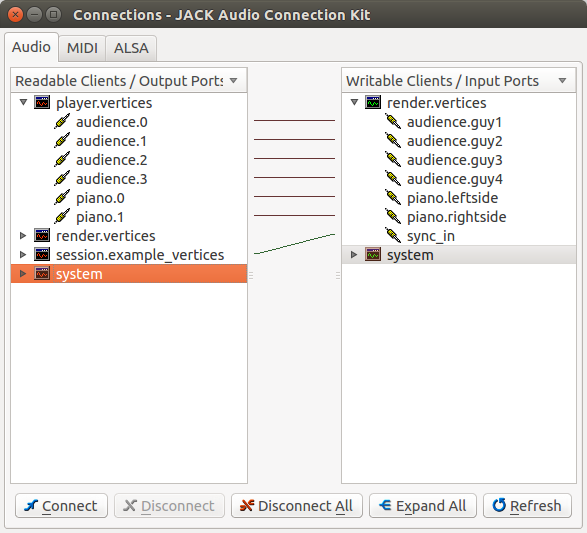
\includegraphics[width=0.8\textwidth]{connectsounds.png}}
  \caption{Connections, which are created, when using attribute
    \attr{connect} in the element \elem{sound}.}
  \label{fig:connect}
\end{figure}
 
Figure \ref{fig:vertices} presents an example of a scene containing sound sources
consisting of more than one sound vertex.

\begin{figure}[htb]
  \centering
  \fbox{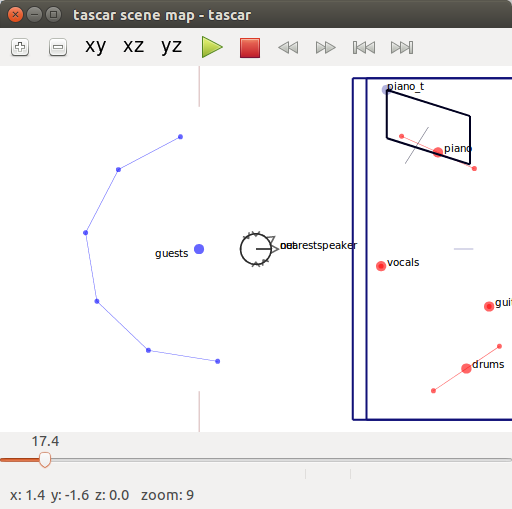
\includegraphics[width=0.8\textwidth]{jazzclub.png}}
  \caption{Examples of sound sources and their vertices. In this scene
    there are point sources like "vocals" or "guitar". There are also
    sound sources with more than one vertex like "guests" (6 vertices)
    or "piano" (2 vertices) - the big dot close to the name of the
    source is the reference point for a given source.}
  \label{fig:vertices}
\end{figure}

Source directivity is defined by the source module types. Currently
the types ``omni'', ``cardioidmod'' and ``door'' are supported.

\subsubsection{Source directivity ``omni''}

The ``omni'' source directivity has no configuration variables. The
sound source radiates independently of the direction.

\subsubsection{Source directivity ``cardioidmod''}

The ``cardioidmod'' source directivity has these attributes:
\begin{tscattributes}
\indattr{f6db} & Frequency in Hz, at which a 6~dB attenuation at 90 degrees is achieved (default: 1000) \\
\indattr{fmin} & Low-end limit for stabilization (default: 60)                                          \\
\end{tscattributes}
At low frequencies, the source radiates omni-directionally. At higher
frequencies, a cardioid-like radiation pattern is achieved.

\subsubsection{Source directivity ``door''}

The ``door'' source directivity has these attributes:
\begin{tscattributes}
\indattr{width} & Door width in meters (default: 1)\\
\indattr{height} & Door height in meters (default: 2)\\
\indattr{falloff} & Distance at wich the gain attenuation starts (default: 1)\\
\indattr{distance} & Distance by which the source is shifted behind the door (default: 1)\\
\indattr{wndsqrt} & Flag to control von-Hann fall-off (false, default) or square-root of von-Hann fall-off (true)\\
\end{tscattributes}
Door sources shift the perceived source position behind a ``door''
shape, limited by the edges. They are basically designed for
interactive transitions between simulated rooms.


\subsubsection{The {\tt <sndfile .../>} element}\label{sec:sndfile}\index{sndfile}\index{sound file}

\paragraph{Note} Under high CPU load and for long files, due to a yet unidentified racing condition in rare cases the time offset might be wrong. Thus it is recommended to use the audio plugin \elem{sndfile} instead (Section \ref{sec:ap_sndfile}).

A sound content can be assigned to a diffuse sound field using a child
element \elem{sndfile}.
%
The child element \elem{sndfile} has an attribute \attr{name}, where we
specify sound file, which we would like to associate with the source.
%
In the previous example we assign a file \textit{clock.wav} to a sound
source called "clock".

Each time we use the element \elem{sndfile}, new jack input ports
called \verb!player.<scenename>:<objectname>.<channel>! will be
created (one for each audio channel in the sound file), e.\,g.\ here
it would be \verb!player.scene_example_kitchen:clock.1!, because
\textit{clock.wav} has a single audio channel (mono).
%
The sound file will be played back by the player part.  
%
If there are more than one sound files assigned to a source object,
they will appear as different channels in audio player (according to
the order in the scene definition). The first sound file in the scene
definition has by default the number 0.

In practice, we assign more than one sound file to a source if the
source consist of more than one sound vertex, so then each vertex
"plays" the different sound file. 
%
Sound vertices will be discussed in the next section.

\begin{figure}[htb]
  \centering
  \fbox{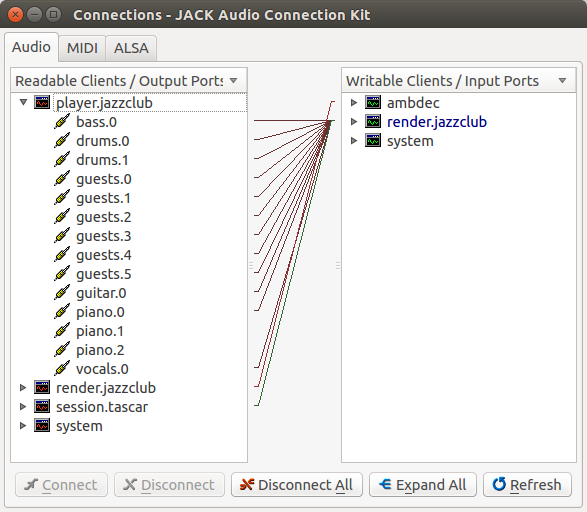
\includegraphics[width=0.8\textwidth]{player.png}}
  \caption{Jack audio player shows different sounds assigned to
    source objects. If there is more than one sound files assigned to
    one source object, then they will have a different channel
    number, starting by default with zero (for example source object
    called guests - we have 6 different sound files assigned to
    this source in the scene definition).}
  \label{fig:player}
\end{figure}


%There can be more than one sound file assigned to a source, for example if we want to change the sound assigned to a source while the scene is played back. We can do it as shown below:

%\begin{verbatim}
 %...
    %<source name="vocals" mute="false" solo="false" color="#ff0000" start="0" end="0">
      %<position interpolation="cartesian">0 2.2 -0.3 2.1</position>
      %<sndfile name="../tascar_scenes/pointsources/jazzclub-vocals_man.wav"  starttime="4" loop="1" gain="-10"/>
      %<sndfile name="../tascar_scenes/pointsources/jazzclub-vocals_woman.wav"  starttime="6" loop="1" gain="-10"/>
      %<sound name="1" connect="@.0"/>
    %</source>
%...

%\end{verbatim}

%We can see that there is now an attribute "starttime" added to a sub-element \textit{sndfile}. The time is specified in seconds and it is counted with respect to the time when the source starts to be active.  

%More than one sound file is sometimes needed if we have a source with more than one sound vertex and we want each vertex to "play" a different sound.

%Each time we use \textit{sndfile} element within one source object, a new jack output port (player) will be created. !!!!!!!!!!!!!!!!!!!!!!!!!!!!!!!!!!!!!!!!!!!!!

\subsection{The {\tt <diffuse .../>} element}\label{sec:diffuse}\index{diffuse}\index{diffuse}

\begin{tscattributes}
\indattr{connect} & Jack connection of ports.                                          \\
\indattr{gain}    & Output gain in dB                                                  \\
\indattr{size}    & Size of box in which the diffuse sound field is audible; default: 1 1 1 \\
\indattr{falloff} & Length of Hanning ramp outside the box in m; default: 1            \\
\end{tscattributes}

\begin{tscelements}
\refelem{position}, \refelem{boundingbox},\refelem{orientation}, \refelem{creator}, \refelem{sndfile}, \elem{plugins}
\end{tscelements}

Apart of sound sources which consist of one or more sound vertices, we
also have a possibility to create diffuse sound fields which ``fill''
the space and are equally loud within a given volume (for example
isotropic babble noise in a cafeteria, or remote traffic). 
%
We can define a diffuse sound field in the following way:
\tscexample[linerange={15-18},firstnumber=15]{example_cashdesk}
%What are the connections in this example?
    
Sound files used to create diffuse sound fields should contain 4 channels
(B format, FuMa normalization). 
%
With attribute \attr{size="x y z"} we can specify the dimensions of
the box in which the diffuse sound field is audible. 
%
To provide a smooth decay of the diffuse sound field, there is a von-Hann
ramp for the gain of the source outside the box. 
%
The length of the ramp can also be specified using
\attr{falloff="..."}.
%
 As all other objects, diffuse sound fields also have position and
orientation, which refers to a position and orientation of the box.


If a port connection is provided (\attr{connect} attribute), then the
four renderer input ports (which are always generated with the diffuse
sound field: \verb!render.<scenename>:<objectname>.n!) are connected
to the audio player output ports \verb!@.0!, \verb!@.1!, \verb!@.2!
and \verb!@.3!, where ''@'' is \verb!player.<scenename>:<objectname>!
.
%


An example on how to add the \elem{addsndfile} audio plugin to a
diffuse sound field can be found below:
%
\tscexample[linerange={5-9},firstnumber=5]{example_diffuse}

The input signal of diffuse sound fields is the B-format (Furse-Malham
normalization, channel order wxyz). For level metering, the RMS level
of the w-channel is taken.


\subsection{The {\tt <receiver .../>} element}\label{sec:receiver}\index{receiver}

A receiver\index{receiver} object can be imagined as a virtual
microphone\index{virtual microphone}\index{microphone}, which captures
the sound in the virtual space, and serves as an output of the virtual
acoustic environment.
%
The choice of the receiver type depends on the playback system and the
desired rendering method.
%
It captures the signal of all sound sources in the scene and computes
these signals according to its type.
%
We can route the output signals to playback system, e.g., loudspeakers
or headphones.

\begin{tscattributes}
\indattr{connect}      & Connection to jack port                                                                  \\
\indattr{gain}         & Gain of jack port in dB; default: 0                                                      \\
\indattr{type}         & Receiver type (see below for a list of receiver types)                                   \\
\indattr{volumetric}   & Size of box for volumetric rendering (x,y,z in m); default: 0 0 0            \\
\indattr{avgdist}      & Average distance which is assumed inside receiver boxes, or 0 to use $(\frac18 V)^{1/3}$ \\
\indattr{point}        & Render point sources (true|false); default: true                                         \\
\indattr{image}        & Render image sources (true|false); default: true                                         \\
\indattr{ismmin}       & Minimal ISM order to be rendered (0)                                                     \\
\indattr{ismmax}       & Maximal ISM order to be rendered ($2^{32}$)                                              \\
\indattr{layers}       & List of active layers, or empty for all layers (default)                                 \\
\indattr{layerfadelen} & Fade length after layer activation or deactivation                                       \\
\indattr{diffuse}      & Render diffuse sound fields (true|false); default: true                                  \\
\indattr{diffusegain}  & Gain applied to diffuse sound fields in dB; default: 0                                   \\
\indattr{falloff}      & Length of Hanning ramp in m, or -1 for normal distance model; default: -1                \\
\indattr{caliblevel}   & Calibration level in dB; default: 93.9794                                                \\
\indattr{delaycomp}    & Subtract this value from delay in delayline (given in seconds)                           \\
\end{tscattributes}

\begin{tscelements}
\refelem{speaker}, \refelem{boundingbox}, \refelem{position},
\refelem{orientation}, \refelem{creator}
\end{tscelements}

A receiver encodes the signals of primary sources, image sources and
diffuse sound fields into a receiver type specific output format. Each
receiver owns one jack output port for each output channel $n$; the
number of channels $N$ depends on the receiver type and
configuration. The output signal of a receiver is
$\mathbf{z}(t)=\left(z_1\left(t\right),z_2\left(t\right),\dots,z_N\left(t\right)\right)$.

The receiver functionality can be split into a {\em panning} or
directional encoding of primary and image sources, and a {\em
  decoding} of first order Ambisonics diffuse signals:
\begin{equation}
\mathbf{z}(t) = 
\underbrace{\sum_{k=1}^K \mathbf{w}(\mathbf{p}_{k,rel}) y_k(t)}_\text{panning} + 
\underbrace{\sum_{l=1}^L \mathbf{D}\hat{\mathbf{O}}_{rec}\hat{\mathbf{O}}^{-1}_{src}\mathbf{f}_l(t)^T}_\text{diffuse decoding}
\end{equation}
In the panning part, the driving weights
$\mathbf{w}=(w_1,w_2,\dots,w_N)$ depend on the relative source
position in the receiver coordinate system,
$\mathbf{p}_{rel}=\mathbf{O}_{rec}^{-1}\left(\mathbf{p}_{src}-\mathbf{p}_{rec}\right)$. For
the definition of the receiver orientation matrix $\mathbf{O}_{rec}$
see Eq.\ \ref{eq:orientation} on page
\pageref{eq:orientation}. $y_k(t)$ is the output signal of the
acoustic model, i.e., distance-dependent gain and air absorption, for
the $k$-th source; $K$ is the number of all primary and image
sources. In the diffuse decoding part, $\mathbf{D}$ is the receiver
type specific first order Ambisonics decoding matrix,
\begin{equation*}
\mathbf{D} = \left(
\begin{array}{cccc}
  d_{1,w} & d_{1,x} & d_{1,y} & d_{1,z} \\
  \vdots    & \vdots  & \vdots  & \vdots  \\
  d_{n,w}  & d_{n,x} & d_{n,y} & d_{n,z}
\end{array}\right)\text{,}
\end{equation*}
and $\hat{\mathbf{O}}_{rec}$is the rotation matrix for first order
Ambisonics signals, to compensate the receiver orientation (see
Eq.\ \ref{eq:foarot}, page \pageref{eq:foarot}). $\mathbf{f}_l$ is the
first order Ambisonics signal of the $l$-th diffuse sound field; $L$ is the
number of all diffuse sound fields, including diffuse reverberation inputs.

For all speaker based receiver types, $D$ is a first order Ambisonics
decoder matrix, with optional speaker density compensation and
decorrelation filters. To achieve a $\max rE$-decoder, set the
attribute \indattr{xyzgain} to 0.707 for regular horizontal speaker
layouts and to 0.577 for regular 3D speaker layouts.  For Ambisonics
based receiver types, $D$ is a diagonal matrix.
%
By default, the decoded output of the first order Ambisonics rendering
is decorrelated using FIR all-pass filters to achieve diffuse sound
fields and avoid coloration artifacts (see \indattr{decorr} and
\indattr{decorr\_length} for details).

Figure \ref{fig:renderer} presents the typical connections in \tascar{}
and may help to visualize the role of the receiver.

\begin{figure}[htb]
  \centering
  \fbox{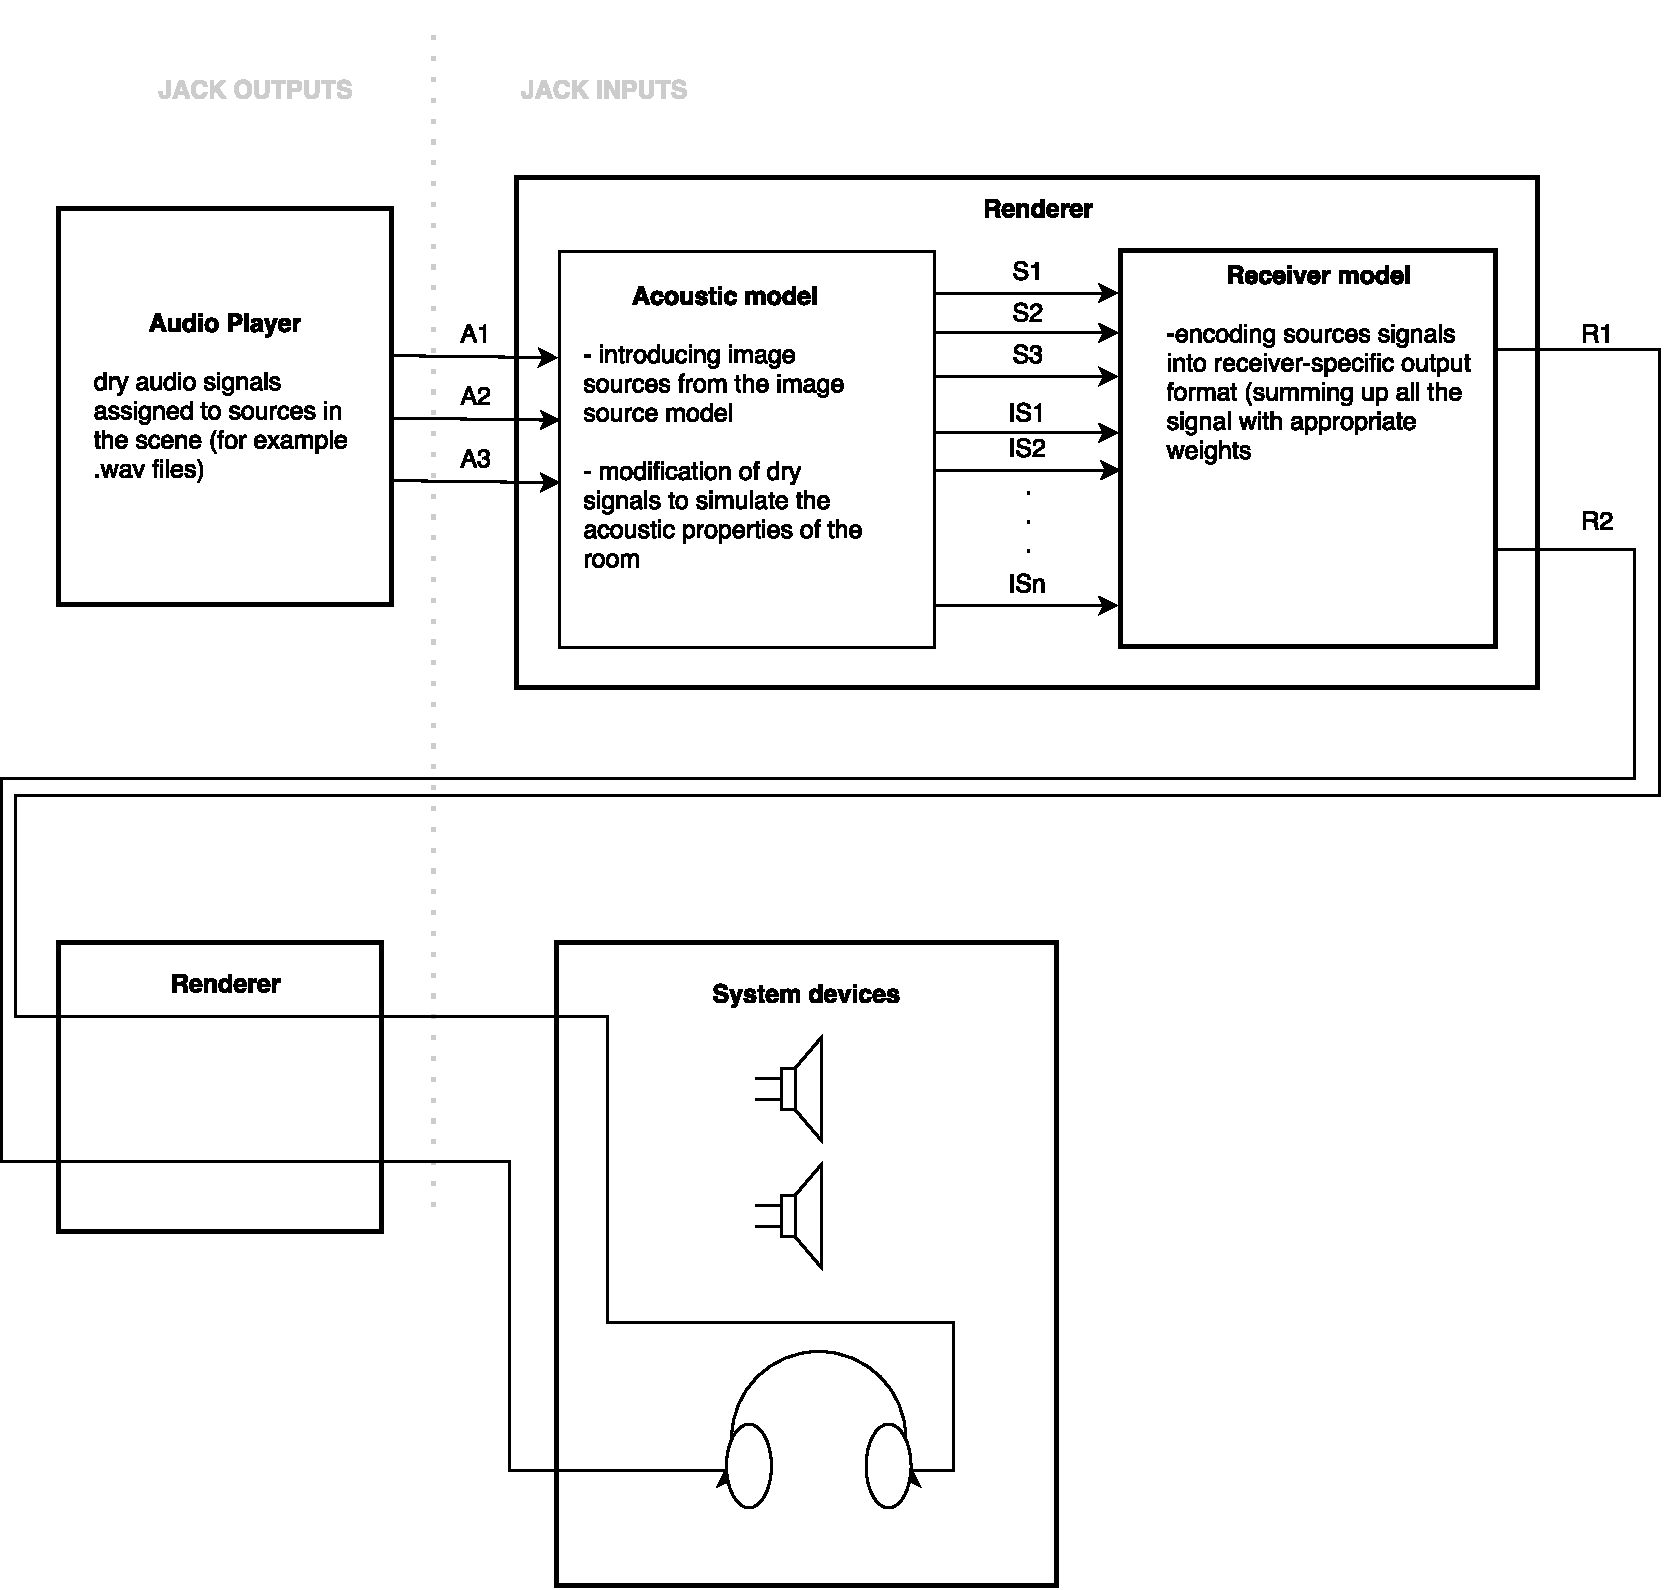
\includegraphics[width=0.8\textwidth]{renderer}}
  \caption{Typical structure of connections in \tascar{}.}
  \label{fig:renderer}
\end{figure}

If the \attr{volumetric} attribute defines a non-zero volume, then all
sources within the receiver volume box are rendered with the same
gain (volumetric rendering).
%
An average distance of $(\frac18 V)^{1/3}$ with the volume $V$ is
assumed, or if \attr{avgdist} is provided, then the provided value is
taken.
%
Outside the box either a von-Hann ramp is applied (\attr{falloff}
$>0$), or the standard distance model is applied.
%
With volumetric receiver settings, the delay will depend on the
relative distance between the receiver origin and the source position.

\subsubsection{The {\tt <speaker .../>} element}\label{sec:speaker}\index{speaker}

The speaker layout of speaker based receiver types can be defined in a
separate layout file specified in the \attr{layout} attribute, in a
list of \elem{speaker} elements within the receiver definition.

\begin{tscattributes}
\indattr{az}         & Azimuth of loudspeaker in degrees (optional; default 0)   \\
\indattr{el}         & Elevation of loudspeaker in degrees (optional; default 0) \\
\indattr{r}          & Distance (optional; default 1)                            \\
\indattr{delay}      & Static delay in seconds (default: 0)                      \\
\indattr{label}      & Additional port label (optional; default empty)           \\
\indattr{connect}    & Connection to jack port                                   \\
\indattr{compB}      & FIR filter coefficients for speaker calibration.          \\
\end{tscattributes}

To activate FIR speaker correction filter, provide the FIR filter
coefficients in the \attr{compB} attribute. Please note that filter
coefficients are specific to the sampling rate, and not automatically
recalculated upon sampling rate changes. The maximal length of the
correction filter is the audio fragment size plus one.

The top-level element of a layout file, \elem{layout}, can be configured with these attributes:
\begin{tscattributes}
\indattr{caliblevel}     & Calibration level in dB; default: 93.9794                                           \\
\indattr{calibdate}      & Calibration date in format YYYY-MM-DD                                               \\
\indattr{xyzgain}        & XYZ-gain for FOA decoding                                                           \\
\indattr{decorr}         & Decorrelate speaker signals in diffuse sound field rendering (default: true)        \\
\indattr{decorr\_length} & Length of decorrelation filter, in seconds (default: 0.05)                          \\
\indattr{densitycorr}    & In diffuse rendering, correct gains locally for loudspeaker density (default: true) \\
\end{tscattributes}

If the caliblevel is provided in the receiver element and the layout
file, then a warning is issued and the value from the layout file is
used. If a calibration date is provided and the calibration is older
than 30 days, a warning is displayed.

%Example:
%
%\tscexample[linerange={5-12},firstnumber=5]{example_neukom}

\subsubsection{receiver types}\index{receiver type}


\begin{table}[htb]
\begin{tabular}{llll}
Type                      & $N$       & panning                                     & diffuse decoding                                                                             \\
\hline
{\tt omni}                & 1         & $w_n=1$                                     & $d_{1,1} = 1$                                                                                \\
{\tt vmic}                & 1         & $w_n=1+a(\tilde p_{rel,x}-1)$                                     & $d_{1,1} = \sqrt{2}(1-a)$, $d_{1,2} = a$                                                                               \\
{\tt cardioid}            & 1         & $w_n=\frac12 \left(\cos(\varphi) + 1\right)$ & $d_{1,1} = 1$                                                                               \\
{\tt ortf} & 2 & ORTF microphone & $\max r_E$\\
{\tt amb\_3h0v}           & 7         & $w_n=\left\{
\begin{array}{cl}
\sqrt{2}                  & n=1                                                                                                                                                    \\
\cos(\frac{n}{2}\varphi)   & n\, \textrm{even}                                                                                                                                     \\
\sin(\frac{n-1}{2}\varphi) & n\, \textrm{odd}
\end{array}\right.$       & $d_{n,n}=1,\, n=\{1,2,3\}$                                                                                                                             \\
{\tt amb\_3h3v}           & 16        &  
$w=
\left(\begin{array}{c}
w_w                                                                                                                                                                                \\w_y\\w_x\\w_z\\w_v\\w_t\\w_r\\w_s\\w_u\\w_q\\w_o\\w_m\\w_k\\w_l\\w_n\\w_p
\end{array}
\right)=
\left(\begin{array}{c}\sqrt{2}                                                                                                                                                     \\
\cos(\theta)\sin(\varphi)                                                                                                                                                          \\ %y
\cos(\theta)\cos(\varphi)                                                                                                                                                          \\ %x
\sin(\theta)                                                                                                                                                                       \\ %z
2 w_x w_y                                                                                                                                                                          \\ %v
2 w_z w_y                                                                                                                                                                          \\ %t
\frac12 (3 w_z^2 - 1)                                                                                                                                                              \\ %r
2 w_z w_x                                                                                                                                                                          \\ %s
w_x^2 - w_y^2                                                                                                                                                                      \\ %u
(3 w_x^2 - w_y^2) w_y                                                                                                                                                              \\%q
2.598076 w_z w_v                                                                                                                                                                   \\ %o
0.726184 (5 w_z^2 - 1) w_y                                                                                                                                                         \\ %m
\frac12 w_z (5 w_z^2 - 3)                                                                                                                                                          \\ %k
0.726184 (5 w_z^2 - 1) w_x                                                                                                                                                         \\ %l
2.598076 w_z w_u                                                                                                                                                                   \\ %n
(w_x^2 - 3 w_y^2) w_x                                                                                                                                                              \\ %p
\end{array}\right)$   & $d_{n,n}=1,\, n=\{1,2,3,4\}$                                                                                                                               \\
{\tt neukom\_basic}   & user def. & $w_n=1+2\sum_{l=1}^{order}\cos(l\varphi_n)$                                                                                                    \\
{\tt neukom\_inphase} & user def. & $w_n=\cos(0.5\varphi_n)^{order}$                                                                                                               \\
{\tt hoa2d}           & user def. & see \cite{Daniel2001} for details.                                                                                                             \\
{\tt nsp}             & user def. & $w_{\argmin\left\{\norm[\big]{\frac{\mathbf{p}_{rel}}{\norm{\mathbf{p}_{rel}}} - \frac{\mathbf{p}_{spk}}{\norm{\mathbf{p}_{spk}}}}\right\}}=1$ \\
{\tt hann}            & user def. & $w_n = \left(\frac12 + \frac12 \cos\left(\min\left\{\left|\frac{N}{2} \varphi_n\right|,\pi\right\}\right)\right)^\gamma$                       \\
{\tt vbap}, {\tt vbap3d}            & user def. & see \cite{Pulkki1997} for details.                                                                                                             \\
%{\tt vbap3d}         & user def. & $ w_n=?$ & $d=?$                                                                                                                               \\
\end{tabular}
\caption{Specification of receiver types. $d_{n,wxyz}=0$ except for
  the given entries. $(\varrho,\varphi,\theta)$ is the source position
  in spherical coodinates in the receiver coordinate
  system. $\varphi_n$ is the azimuthal angular distance between
  loudspeaker $n$ and the sound source.}\label{tab:receivers}
\end{table}

There are following types of receivers (see Table \ref{tab:receivers} for an overview):

\paragraph{omni-directional:}

\begin{lstlisting}[numbers=none]
<receiver type="omni"/>
\end{lstlisting}

If we use the simple omni-directional receiver, then sources coming
from all directions are rendered with the same weight $w=1$ and at the
output of the renderer we will get just one channel, $N=1$ - the
summation of sources from all directions:

$N=1$,
$w_n=1$

\paragraph{virtual microphone:}

\begin{lstlisting}[numbers=none]
<receiver type="vmic" a="0"/>
\end{lstlisting}

The virtual microphone receiver type has a single output channel. The
driving weight is
\begin{equation}
w = 1 + a (\tilde{p}_{rel,x} - 1).
\end{equation}
It's directivity pattern can be controlled between omni-directional and
figure-of-eight with the directivity coefficient $a$; with $a=0$ this
is an omni-directional microphone, with $a=\frac12$ a standard
cardioid, and with $a=1$ a figure-of-eight.
%
The diffuse decoding matrix is
\begin{equation}
\mathbf{D} = \left( \sqrt{2}(1-a) \quad a \quad 0\quad  0 \right).
\end{equation}
The factor \(\sqrt{2}\) of the \(w\)-channel is needed to account for
the Furse-Malham normalization of the diffuse signals.

\paragraph{cardioidal:}

\begin{lstlisting}[numbers=none]
<receiver type="cardioid"/>
\end{lstlisting}
  
If we use a cardioidal receiver, then sources are multiplied with a
different weight (depending on the direction of arrival, according to
cardioidal directivity pattern) and at the output of the renderer we
will also get just one channel - a summation of sources coming from
different directions multiplied with different weights.
 
$N=1$, $w_n=\frac{1}{2}(cos(\alpha) +1)$,\\
where \(w(n)\) depends on
the angle between the source and the receiver, $\alpha$ (direction
from which the source is coming).

\paragraph{virtual ORTF stereo microphone}\index{ORTF stereo microphone}\index{stereo}
 
\begin{lstlisting}[numbers=none]
<receiver type="ortf" f6db="3000" fmin="80" distance="0.17" angle="110"/>
\end{lstlisting}

This receiver implements a classical ORTF stereo microphone
technique. The cardioid microphone pattern has a frequency dependency;
the 6~dB cutoff frequency for 90 degrees is given by the attribute
\indattr{f6db}. The attribute \indattr{fmin} defines the cutoff
frequency for 180 degree sounds. The attributes \indattr{distance} and
\indattr{angle} control the microphone geometry.

Typical values for small diaphragms are \attr{f6db="3000"} and
\attr{fmin="800"} (these are the default values since version
0.172.2); for a higher directivity, use \attr{f6db="1000"} and
\attr{fmin="60"} (default values of earlier versions).

\paragraph{first order ambisonics:}

Horizontal FOA:
\begin{lstlisting}[numbers=none]
<receiver type="amb1h0v"/>
\end{lstlisting}

Full periphonic:
\begin{lstlisting}[numbers=none]
<receiver type="amb1h1v"/>
\end{lstlisting}

The normalization attributes \attr{normalization="FuMa"} (default) or
\attr{normalization="SN3D"} are supported.

\paragraph{third order ambisonics:}

Horizontal HOA:
\begin{lstlisting}[numbers=none]
<receiver type="amb3h0v"/>
\end{lstlisting}
$N=7$, $w_k=\left\{
\begin{array}{cl}
\sqrt{2} & k=0\\
\cos(\frac{k+1}{2}\alpha) & k\, \textrm{odd}\\
\sin(\frac{k}{2}\alpha) & k\, \textrm{even}
\end{array}\right.
$

Full periphonic:
\begin{lstlisting}[numbers=none]
<receiver type="amb3h3v"/>
\end{lstlisting}
  
Receiver of this type will produce ambisonics output channels - 7
channels for \lstinline!type="amb3h0v"! and 16 channels for
\lstinline!type="amb3h3v"!. Each channel corresponds to different
directivity pattern, so the resulting signal will be calculated for
each channel differently.

%, for example channel "u" is calculated with
%the following weights:
%  
% \( C_U=\frac{1}{N}\displaystyle\sum_{i=1}^{N}w_N S_N \) with \(w_N=S_N \cos(2\*\phi)cos^2(\theta)\)
% 
 
To play back the content of a virtual scene on an arbitrary playback
device, we have to use an external tool to decode the ambisonics
format (a tool which will mix the ambisonics channels signals in an
appropriate way in order to get the signals for channels of our
playback system).  To achieve this, we can make a jack connection
between the output of the ambisonics receiver
(\verb!<scenename>.render:<receivername>.<channel>!) and ambisonics
decoder "ambdec"\index{ambdec}\index{decoder}:
%
\itscexamplepriv[linerange={2-5},numbers=none]{objects}
%
If we use connect="ambdec:in", then the connections will be done, so
that the channels have the same name in both receiver output and
ambdec input, as shown in the Figure \ref{fig:ambdec}. 
%
We can then go to the settings of the ambdec device and find a type of
output corresponding to our playback set up
(Config$>>$Load$>>$usr/share/ambdec/presets). 
%
For example if we choose a preset \textit{octagon-3h0v}, the
appropriate output ports will appear (Figure \ref{fig:ambdec_out}),
which can be than connected with the system playback devices.

\begin{figure}[htb]
  \centering
  \fbox{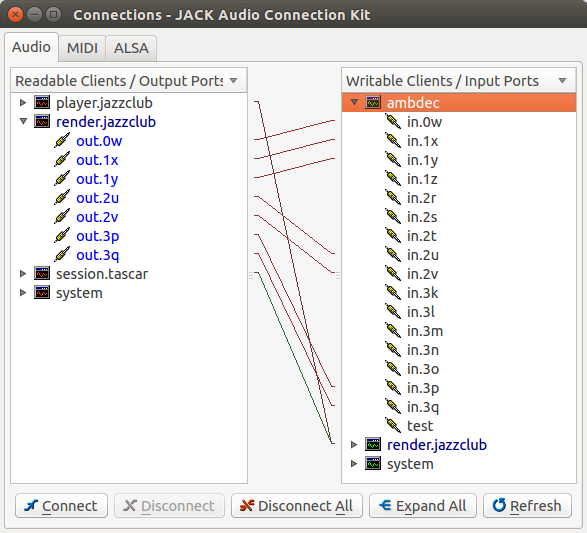
\includegraphics[width=0.8\textwidth]{render_ambdec.png}}
  \caption{Connections, which are created, when using attribute \attr{connect} in the element \elem{sound}}
  \label{fig:ambdec}
\end{figure}
 
 \begin{figure}[htb]
  \centering
  \fbox{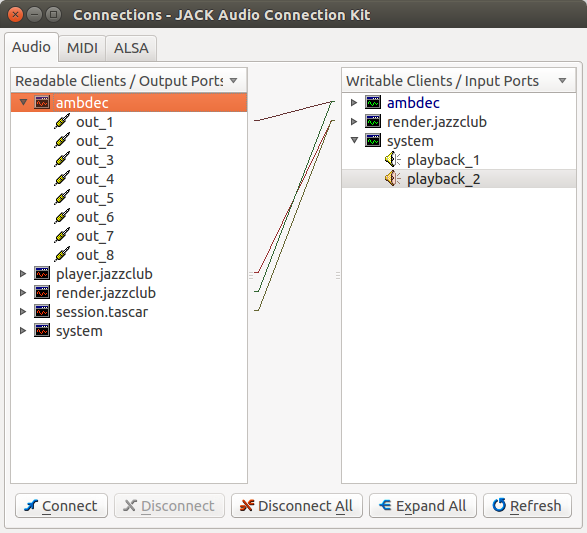
\includegraphics[width=0.8\textwidth]{ambdec_out.png}}
  \caption{Ambdec output ports for a horizontal octagon}
  \label{fig:ambdec_out}
\end{figure}

There are also speaker-based decoding methods (VBAP, ambisonics
panning and nearest-speaker panning) which require the specification
of loudspeakers - together with the receiver type, we define a set of
virtual loudspeakers located relative to the position of this
receiver.
%
Information about the number of loudspeaker and their location is then
exploited to produce appropriate receiver output channels.
%


\begin{figure}[htb]
  \begin{subfigure}[t]{0.25\textwidth}
    \centering
    \fbox{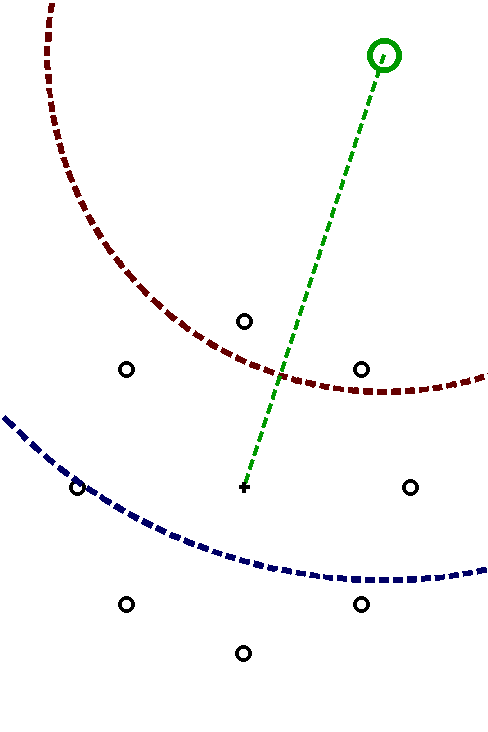
\includegraphics[width=0.85\linewidth]{method_input}}
    \caption{original}
  \end{subfigure}%
  \begin{subfigure}[t]{0.25\textwidth}
    \centering
    \fbox{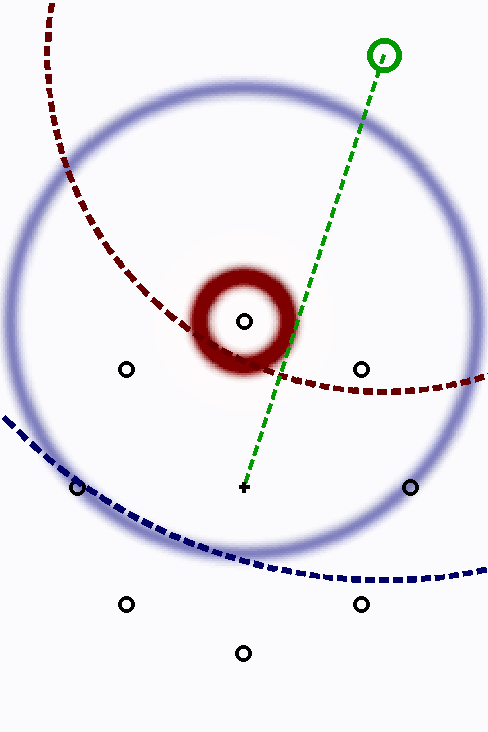
\includegraphics[width=0.85\linewidth]{method_nsp}}
    \caption{nsp}
  \end{subfigure}%
  \begin{subfigure}[t]{0.25\textwidth}
    \centering
    \fbox{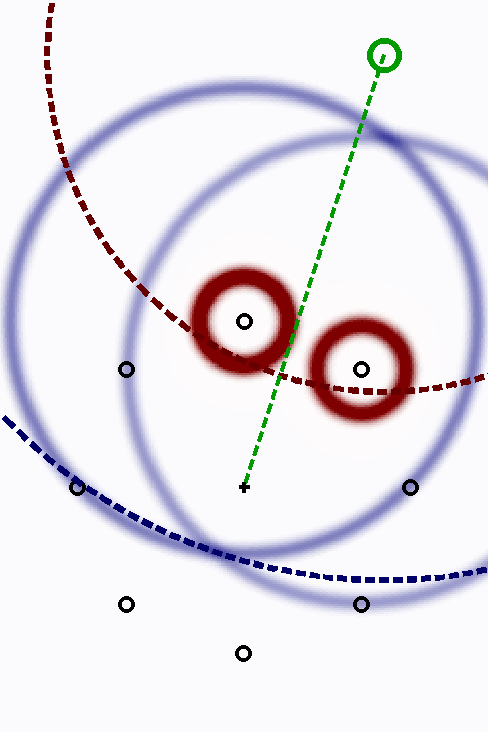
\includegraphics[width=0.85\linewidth]{method_vbap}}
    \caption{vbap}
  \end{subfigure}%
  \begin{subfigure}[t]{0.25\textwidth}
    \centering
    \fbox{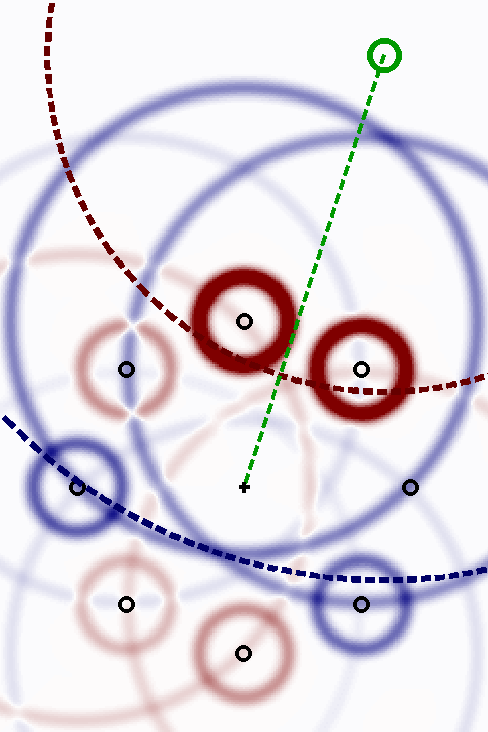
\includegraphics[width=0.85\linewidth]{method_amb_basic}}
    \caption{hoa2d}
  \end{subfigure}
  %\centering
  %\fbox{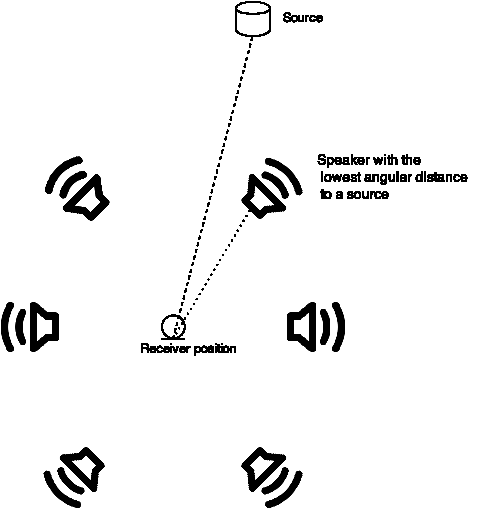
\includegraphics[width=0.8\textwidth]{nearest.pdf}}
  \caption{Schematic representation of the reproduced sound fields
    with different reproduction methods..}
  \label{fig:repromethods}
\end{figure}


\paragraph{2D higher order Ambisonics \citep{Daniel2001}:}\index{hoa2d} 

\begin{lstlisting}[numbers=none]
<receiver type="hoa2d" order="3" maxre="true">...</receiver>
\end{lstlisting}

This receiver type provides horizontal higher order ambisonics with
basic or $\max r_E$ decoding.
%
If \attr{order} is zero or unset, then the maximum possible order for
the given number of loudspeakers is used.

\begin{tscattributes}
\indattr{order}            & Ambisonics order; 0: use maximum possible (default: 0)                                                                      \\
\indattr{rotation}         & Rotation of the loudspeaker array in degrees (default: compensate average speaker rotation)                                 \\
\indattr{maxre}            & Use $\max r_E$ decoder (true) or basic decoder (false) (default: false)                                                     \\
\indattr{diffup}           & Use diffuse upsampling similar to \citet{Zotter2014} (default: false)                                                       \\
\indattr{diffup\_rot}      & Decorrelation rotation in degree (default: 45)                                                                              \\
\indattr{diffup\_delay}    & Decorrelation delay in seconds (default: 0.01)                                                                              \\
\indattr{diffup\_maxorder} & Maximum order of diffuse sound fields (default: 100)                                                                        \\
\indattr{filtershape}      & De-correlation filter shape for source width encoding, one of ``none'' (default), ``notch'', ``sine'', ``tria'', ``triald'' \\
\indattr{filterperiod}     & Filter period in seconds for source width encoding (default: 0.005)                                                         \\
\end{tscattributes}

\paragraph{Note:}
Only regular speaker arrays can be used. Explicit speaker
distributions are ignored, and a regular speaker distribution with
counter-clockwise azimuths is assumed, with the first speaker starting
at the value provided in the \attr{rotation} attribute.
%
If the \attr{rotation} attribute is not given, then the average
difference between a regular layout and the explicit speaker azimuth
is taken as \attr{rotation}.

If \indattr{diffup} is set to ``true'', diffuse-decoding is using the
internal decoder, which is also used for decoding of panned sources.
%
If \indattr{diffup} is set to ``false'', the standard speaker-based
diffuse render method is applied.
%
Source-width encoding splits the signal into two uncorrelated signals
and creates virtual sound sources separated by the source width.

An alternative receiver type \verb!hoa2d_fuma! can be used to return
the encoded signal in FuMa normalization and ACN channel order.

\paragraph{Ambisonic panning \citep{Neukom2007}:}

\begin{lstlisting}[numbers=none]
<receiver type="neukom_basic" order="3">...</receiver>
\end{lstlisting}
\begin{lstlisting}[numbers=none]
<receiver type="neukom_inphase" order="3">...</receiver>
\end{lstlisting}

With these types of receivers, we can also use the ambisonics surround
format for creating an appropriate sound for our playback system. 
%
This time however, we don't have to use an external tool to decode the
ambisonics format. 
%
It will be done automatically after we specify the positions of of the
playback channels using element \refelem{speaker} (which is equivalent
to choosing an appropriate preset in the ambdec tool). 
%
%It can be done in the following way:
%\tscexample[linerange={5-13},firstnumber=5]{example_neukom}

Above we can see, that speakers are defined with the element
\refelem{speaker} and their position and orientation is defined with
attributes \attr{el}, \attr{az} and \attr{r} and is relative to the
position and orientation of the whole receiver object.
%
Output channels defined using element \refelem{speaker} will appear in
the Jack Audio as an output of the rendering stage.
    

%difference between basic and inphase???

\paragraph{nearest speaker receiver:}

\begin{lstlisting}[numbers=none]
<receiver type="nsp"><speaker az="0"/>...</receiver>
\end{lstlisting}
Another speaker-based decoding method is the nearest-speaker
receiver. 
%
This receiver also requires defining the position of the playback
channels and we can do it in the following way (see
\verb!example_nearest.tsc!):
\tscexample[linerange={4-7},firstnumber=4]{example_nearest}

\tscexampleext[linerange={2-7},firstnumber=2]{nsp.spk}

If we load a scene with such a receiver in \tascar{}, we will see all the
specified channels as an output of the rendering stage in the Jack
Audio. 
%
However, this time, for each source there is only one channel which is
active, i.e. the one for which there is the lowest angular distance
from the loudspeaker to the source.


\paragraph{von-Hann window panning:}


\begin{lstlisting}[numbers=none]
<receiver type="hann" wexp="0.5">...</receiver>
\end{lstlisting}
If $N$ speakers are defined, $\alpha$ is the angle between a speaker
$k$ and the virtual sound source, and $\gamma$ is the window exponent
(\indattr{wexp}), then the speaker gain $g_k$ is
\begin{equation}
w_k = \left(\frac12 + \frac12 \cos\left(\frac{N}{2} \alpha\right)\right)^\gamma
\end{equation}


%\label{sec:speaker}%
\paragraph{Vector base amplitude panning \citep{Pulkki1997}:}\index{vbap} 

\begin{lstlisting}[numbers=none]
<receiver type="vbap" layout="spkeaker.spk"/>
\end{lstlisting}

\begin{lstlisting}[numbers=none]
<receiver type="vbap3d" layout="spkeaker3d.spk"/>
\end{lstlisting}

\paragraph{intensityvector:}

This specialized receiver type accumulates the sound intensity
weighted direction. This receiver type is used only for analysis and
characterization of acoustic scene properties. Its only attribute is
the intensity integration time constant \indattr{tau}, measured in
seconds, with the default value of 0.125.

\subsection{Reflectors: {\tt <face .../>} and {\tt <facegroup .../>} elements}\label{sec:face}\label{sec:facegroup}\index{face}\index{facegroup}

The \elem{face} element defines a single reflecting surface.

\begin{tscattributes}
\indattr{width}, \indattr{height}         & Dimension of reflector in meters; default: 1                                       \\
\indattr{reflectivity}, \indattr{damping} & First order low pass filter coefficients                                           \\
\indattr{edgereflection}                  & Apply edge reflection in case of not directly visible image source (default: true) \\
\indattr{vertices}                        & List of Cartesian coordinates to define polygon surface                            \\
\end{tscattributes}

If the attribute \indattr{vertices} contains at least three
coordinates then a polygon surface is constructed using the vertices
list. 
%
Otherwise, a rectangular surface with the given width and height is
created.
%
The vertices of the reflector are at $(0,0,0)$, $(0,w,0)$, $(0,w,h)$
and $(0,0,h)$. The face normal, i.e., the reflecting side of the
surface, is pointing in positive $x$-axis.

%
In \verb!example_reflectors.tsc! both cases are shown:
\tscexample[linerange={4-11},firstnumber=4]{example_reflectors}

The \elem{facegroup} element creates a group of polygon reflectors,
with common reflection properties.

\begin{tscattributes}
\indattr{reflectivity}, \indattr{damping} & First order low pass filter coefficients                                           \\
\indattr{importraw}                       & File name of raw file containing list of polygon surfaces                          \\
\indattr{shoebox}                         & Dimension of a shoebox shaped room with inward-facing walls (default: ``0 0 0'')   \\
\indattr{edgereflection}                  & Apply edge reflection in case of not directly visible image source (default: true) \\
\end{tscattributes}

Element \elem{facegroup} behaves also as an object, since it also has
a position and orientation in space. 
%
So if we change the position or orientation of the whole
\elem{facegroup}, it will also relatively change for all the planes
included in the \elem{facegroup}.

We can define a \elem{facegroup} in the following way (see example
\verb!example_reflectors.tsc!):
\tscexample[linerange={12-17},firstnumber=12]{example_reflectors}

First, we define the facegroup with the name, reflectivity as well as
the position and orientation of the whole facegroup. 
%
Then, we use a sub-element \elem{faces} (not the same as \elem{face}
!) to define the surfaces which will be included in the group.
%
Each line has to contain the coordinates x y z for at least three
vertices. 
%
Each surface is defined in one line (by specifying coordinates of the
vertices of a surface). 
%
At this point in the code we shouldn't leave empty lines.

Instead of defining all the surfaces manually, we can also create a
more complicate shape in blender and then export face group raw files
from blender model:
\begin{verbatim}
tascar_blenderexport blendfile.blend
\end{verbatim}
This will export the meshes of all blender mesh objects of the
currently selected scene, or if available, from the scene named
``tascar'', to the file {\tt <blendfilename>\_<objectname>.raw} and
all curve objects to a \tascar{} track file {\tt
  <blendfilename>\_<objectname>.csv}.

When we already have a text file, where the coordinates for all the
vertices are already specified, we can import it to \tascar{} scene
definition using an attribute \indattr{importraw}:
\begin{lstlisting}[numbers=none]
<facegroup name="mirrors" reflectivity="1" damping="0" importraw="filename.raw"/>
\end{lstlisting}

A simple shoebox shaped room can be created by setting the attribute
\attr{shoebox="x y z"} to a finite size.
%
The size is given in $x,y,z$ dimensions. All faces are pointing
inwards.
 
The normal of faces, i.e., the face orientation, is relevant for the
acoustics simulation: Image sources are only active if the primary
source is in the direction of the face normal.

Polygons meshes are flattened by a projection on a plane which is
orthogonal to the polygon normal vector.

\subsection{Obstacles: {\tt <obstacle .../>} element}\index{obstacle}\label{sec:obstacle}

Obstacles are polygon meshes which can absorb sound and create
diffraction at their boundaries. The diffraction pattern is only a
rough approximation.
\begin{tscattributes}
\indattr{transmission} & Amount of transmission                                    \\
\indattr{importraw}    & File name of raw file containing list of polygon surfaces \\
\end{tscattributes}

An example configuration file can be found in the file {\tt example\_obstacle.tsc}.

\subsection{Masks: {\tt <mask ../>} element}\index{mask}\label{sec:mask}

Global masks affect the attenuation in a receiver, based on the receiver position. 
See Figure \ref{fig:masks}.

\begin{figure}[htb]
    \centering
    \fbox{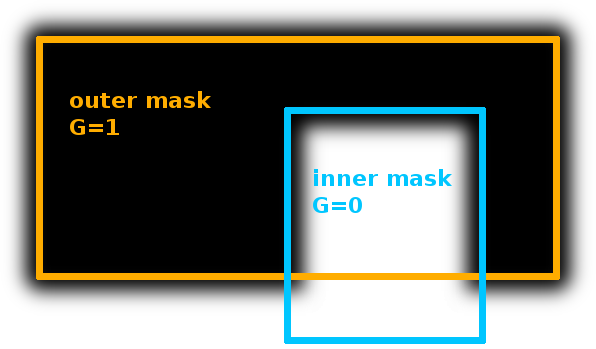
\includegraphics[width=\textwidth]{masks.png}}
    \caption{Global masks example.}
    \label{fig:masks}
\end{figure}

%\begin{figure}[ht]
%\centerline{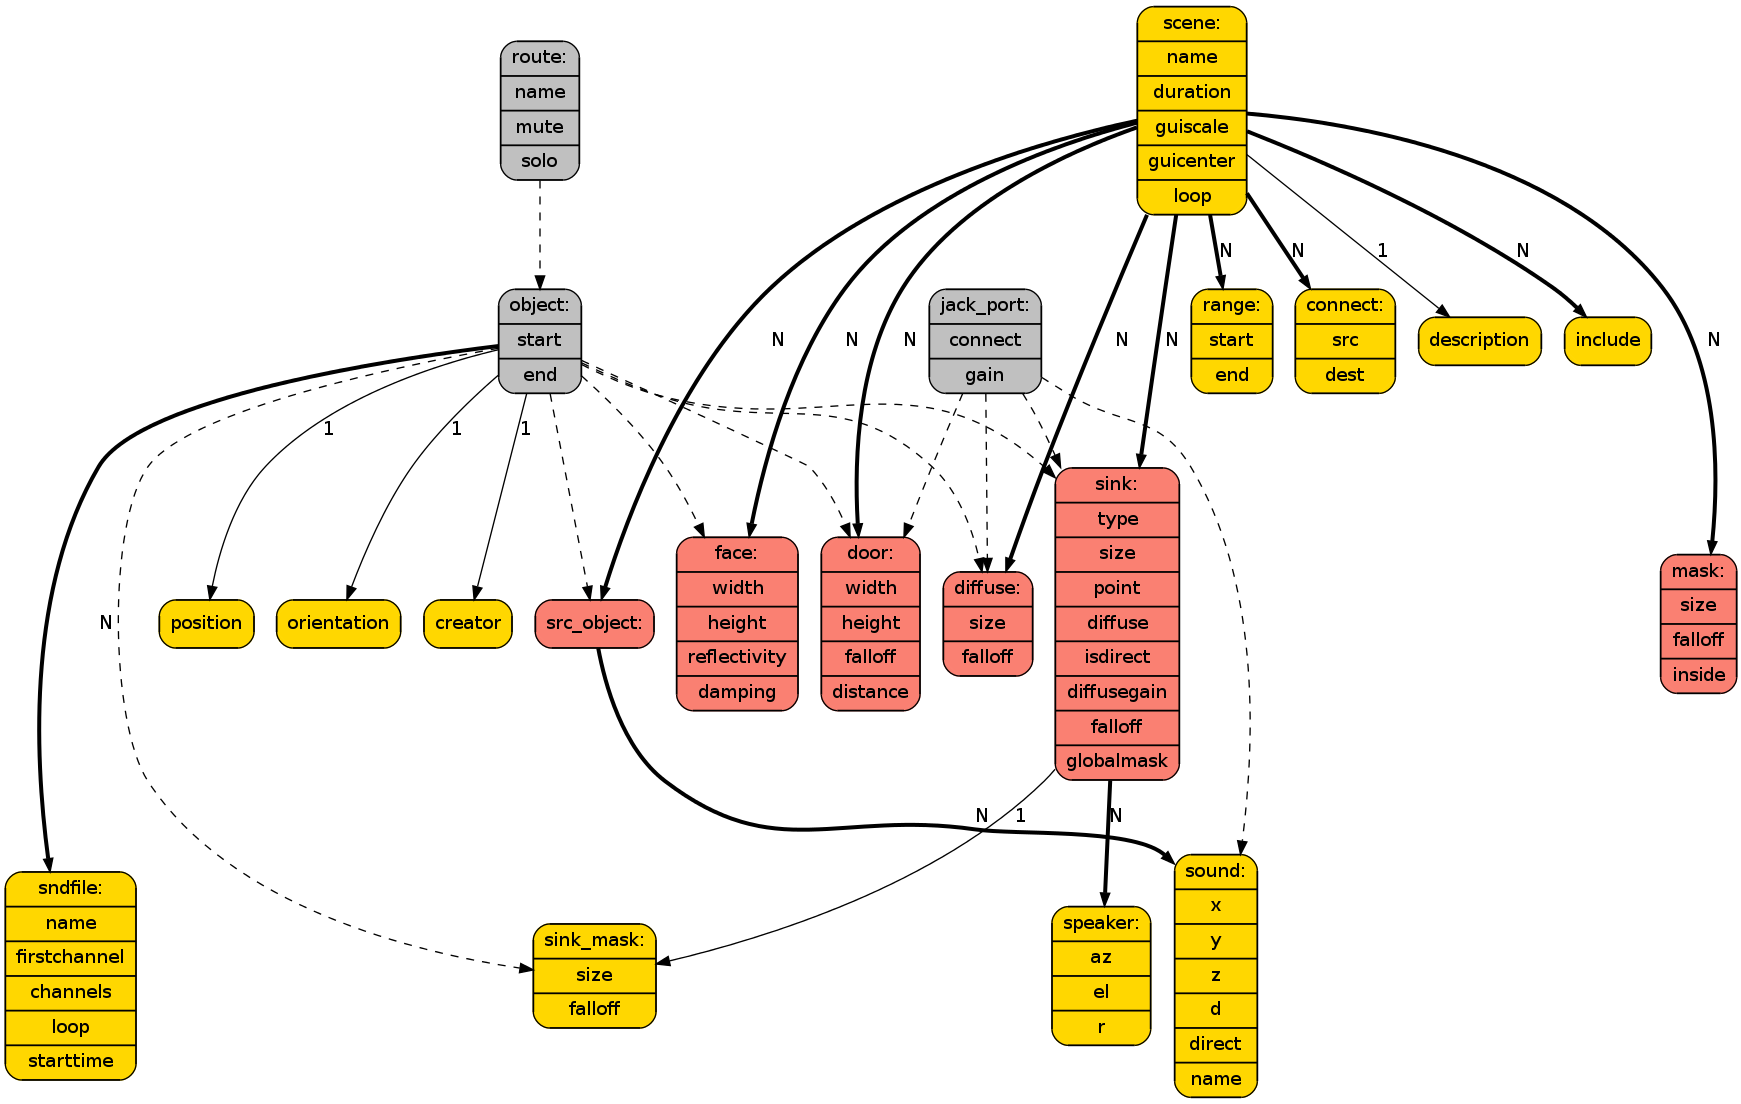
\includegraphics[width=\columnwidth]{filestructure.png}}
%\caption{\label{fig:filestructure}{\it File structure and relations between nodes.}}
%\end{figure}

\clearpage

\section{General purpose modules}\label{sec:module}\index{modules}

External modules which do not directly interact with the acoustic
model of the virtual acoustic environment can be loaded as dynamic
libraries.
%
These modules may analyse or modify the session data, or simply
provide some additional functionality.
%
Modules can be added to a session file within the
\verb!modules!, e.g.,
\begin{lstlisting}[numbers=none]
  <modules>
    <simplecontroller actor="/*/out" ... />
  </modules>
\end{lstlisting}

\input{secmodules.tex}

\section{Actor modules}\label{sec:actormod}

Actor modules can be used in the same way as general purpose modules,
however, their purpose is to change or query the position one or more
objects by using an actor name definition:
\begin{lstlisting}[numbers=none]
<simplecontroller actor="/scene/obj" .../>
\end{lstlisting}
Name matching with \verb!*! is possible. For example, we can choose all the objects from the scene, whose names start with \verb!N!:

\attr{actor="/scene/N*"}

Or if we have more than one scenes, we can choose all the objects called \verb!out! from all scenes:

\attr{actor="/*/out"}

\input{secactmodules.tex}

\clearpage

\section{Audio plugins}\index{Audio plugins}

Each sound vertex \elem{sound}, each diffuse sound field
\elem{diffuse}, and each receiver \elem{receiver} can contain a list
of audio plugins for processing and analysis, such as tone generators
or speech analysis for lip synchronization modeling.
%
These audio plugins are specified within the \elem{plugins} section
within a \elem{sound} or \elem{receiver} element, e.g.:
\tscexample[linerange={9-14},firstnumber=9]{example_audioplugins}
%\begin{lstlisting}[numbers=none]
%<source name="car">
%  <sound name="wheel" z="-0.5">
%    <plugins>
%      <sndfile name="wheelsound.wav" levelmode="rms" level="85"/>
%      <sine f="1000" a="70"/>
%    </plugins>
%  </sound>
%</source>
%\end{lstlisting}

Audio plugins may share their variables via OSC.
%
See the list of OSC variables to check which variables can be
accessed.

Audio plugins are processed in the order they appear in the
configuration within the \elem{plugins} section. For sound vertices,
they are processed before the sound is handed to the acoustic
model. For receivers, audio plugins are processed after the post
processing function of the render format.

\input{secapmodules.tex}

\clearpage

\section{Calibration and level metering}\index{calibration}\index{level}

\tascar{} offers a level meter for each primary or diffuse sound
field and receiver. In the level meters, root-mean-square (RMS)
values in dB SPL, averaged over the past two seconds, are shown.  In
\tascar{}, internal values are measured in Pa. This means that a
sinusoid with an amplitude of one corresponds to a level of 91 dB
SPL. The level of sound sources corresponds to the anechoic free field
level in a distance of 1~m.

Each input port (\refelem{sound} element) and output port
(\refelem{receiver} element) of \tascar{} can be calibrated with the
calibration level attribute \indattr{caliblevel}.

At the input, a full-scale sine wave corresponds to
\attr{caliblevel}$-3$~dB (because the RMS of a sine wave is $-3$ dB).
%
This means that in case of the sine wave, the level of that sound
source is 91 dB SPL, in a 1~m distance and anechoic conditions.
%
The last bit is important: In virtual acoustics we cannot easily
calibrate the level of sound sources at the listening position.
%
In anechoic conditions this can be calculated with the $\frac1r$
amplitude law, but in case of reflections this $\frac1r$ law is not
valid anymore.

For the sine wave the CREST-factor (difference between peak and RMS
level) is 3 dB, but for speech this is roughly 20-24 dB.
%
Thus typically for speech one will need a much higher \attr{caliblevel} than
93~dB, because otherwise a full-scale speech signal would result in
only 70 dB SPL.
%
Typically, any speech test software will have some output calibration value.
%
In case of the Oldenburg Measurement Applications (OMA) this is the
same as the \attr{caliblevel} of \tascar{}.
%
Most likely the value of it will be in the order of 120 dB SPL
(similar to the \attr{caliblevel} of the \tascar{} receiver).
%
If the \attr{caliblevel}-value of the speech test software is known, exactly
the same value should be used for the \tascar{} input \attr{caliblevel}.
%
In that case, the input level meters of \tascar{} should show the same
values as the output level meters of the speech test.

For a calibration of speaker layouts, it is recommended to use the
tool ``tascar\_spkcalib''.

To measure the sound pressure level in a virtual acoustic environment,
one can place an omni-directional microphone at the position of the main
output receiver.
%
This omni-directional level meter should show the same numbers as a
real physical sound level meter in the center of the physical
reproduction system.
%
The sound level meter need to be configured to ``unweighted'',
``Z-weighted'' or ``C-weighted'' settings.
%
Please be aware of the fact that in ``unweighted'' mode the background
noise levels can be in the order of 40-60 dB, due to ventilation of
the room, door slamming in the building, steps, nearby trains and
plains etc., which contain extremely low frequencies.

\subsection{Calibrating speaker layouts with {\tt tascar\_spkcalib}}

All loudspeaker-based rendering methods (e.g., those depending on a
loudspeaker layout file) should result in identical levels at the
listening positions for virtual sound sources from the directions of
the speakers (the levels of interpolated virtual sources may differ
due to differences in the rendering method).
%
The broadband calibration of loudspeaker layouts consists of three
steps: a) calibrate gain differences between loudspeakers b) calibrate
the reference level for point source rendering, and c) calibrate the
gain correction for diffuse sound field rendering.
%
The tool \verb!tascar_splcalib! can be used to perform these steps.

\begin{figure}[htb]
    \centering
    \fbox{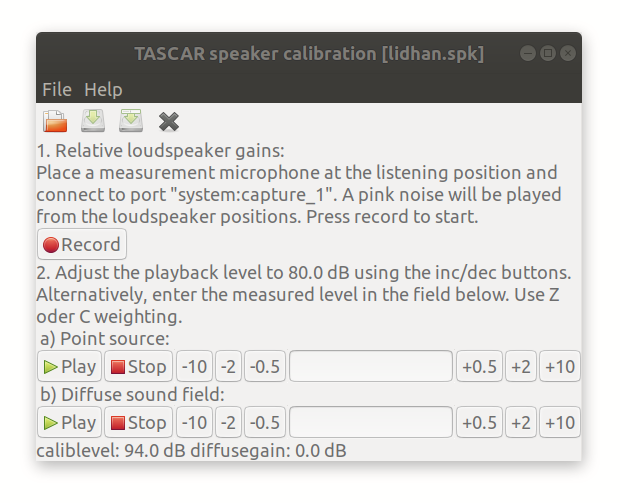
\includegraphics[width=0.7\textwidth]{tascarspkcalib.png}}
    \caption{Loudspeaker calibration window.}
    \label{fig:spkcalib}
\end{figure}

To (re-)calibrate a loudspeaker layout file, open it with
\verb!tascar_splcalib!, e.g., by double-clicking it in the file
explorer.
%
The application has four control areas (see Fig.\ \ref{fig:spkcalib}):
the menu and toolbar at the top of the application window can be used
to open, save and close loudspeaker layout files.
%
Below is the area for measurement of gain differences between
loudspeakers, followed by an area for measurement of the reference
level for point source rendering.
%
At the bottom of the window the area for calibration of the diffuse
rendering gain can be found.

\subsubsection{Calibrating a loudspeaker array for the first time}

The default calibration level in TASCAR is 94~dB SPL. The default test
tone level is 80~dB SPL. If the actual calibration level is far above
the default value, then pressing the ``play'' button will result in
excessive sound levels. Therefore it is recommended to decrease the
sound level by pressing the ``-10 dB'' button several times. Then
press ``play'', and increase the level using the ``+10 dB'', ``+2 dB''
and ``+0.5 dB'' buttons until the level reaches approximately
80~dB. Then press the stop button. From here, follow the instructions
for a re-calibration.

\subsubsection{Re-calibration of a loudspeaker array}

For re-calibration of a loudspeaker array, you will need a measurement
microphone (omni-directional characteristics, flat frequency response
from 60 to 4000 Hz), and a sound level meter with Z or C
weighting. The calibration test tone is a pink noise in the frequency
range from 62~Hz to 4~kHz. Connect the microphone to the port
\verb!system:capture_1! (or change the setting
\verb!tascar.spkcalib.inputport! to the jack port name of your
microphone, see Section \ref{sec:globalconfig} for details), and place
it at the listening position. Now press ``Record'' to start a
recording of levels. The sound will be played from the directions of
the loudspeakers. After the recording is completed, the mean recording
level and its range are displayed next to the ``Record'' button. If
the recording level is very low (below -50 dB), then verify the
connection and configuration of your microphone. Also the level range
should not exceed 20 dB, otherwise inspect the connections of the
loudspeakers.

In the next step, play the test tone as a point source using the
``play'' button in the point source section. Enter the sound pressure
level measured at the listening position into the level entry field in
the window, or use the decrement and increment buttons to adjust the
playback level. When finished with this step, press the ``Stop''
button.

Now, repeat the same procedure, but with a diffuse test sound, by
pressing the ``Play'' button in the diffuse calibration area. Enter
the level reading in the appropriate field, or adjust the level using
the increment/decrement buttons.

If all steps are completed, press the ``Save'' or ``Save as'' button
at the top of the window. The changes are stored into the loudspeaker
file. It is recommended to review the calibration and gain values
using an editor.


\clearpage

\section{Interfacing from MATLAB and GNU/Octave}

For the interface between \tascar{} and MATLAB or GNU/Octave a set of
scripts are provided in \verb!/usr/share/tascar/matlab!.
%
There are the following scripts available:

\subsection{\tt tascar\_ctl}

This function can be used for two basic actions:

\begin{enumerate}
\item Loading a scene, which already exists:
      \verb!h = tascar_ctl('load','filename.tsc')!\\
\item Closing a scene: 
      \verb!h = tascar_ctl('kill',h )!\\

\end{enumerate}

An example of the usage of this (and other MATLAB/GNU Octave functions) can be
found in \verb!example_controlTASCAR.m!.

\subsection{\tt generate\_scene}

In \tascar{}, virtual acoustic environments are defined in an xml file
format.
%
User can write such a file on his own or create it using MATLAB/GNU Octave
function \verb!generate_scene!.
%
This function can generate a simple scene with one speaker based
receiver, N sources distributed on a circle around the receiver and K
virtual loudspeakers, also equally distributed on a circle around the
receiver.
%
There are a couple of parameters which can be specified by a user -
the file name, the number of sources and loudspeakers, radius of the
circle, receiver type, as well as the length of a delayline.



\subsection{\tt tascar\_jackio}

When we already have an xml file with a virtual environment, we may
want to start perfoming some measurements using MATLAB/GNU Octave.
%
The function \verb!tascar_jackio! is used to play and record sound via
jack (jack audio connection kit).
%
It means that we are playing the sound using ports responsible for the
sources in the virtual scene and recording the sound using ports
responsible for the receiver in the scene.
%
Usually, it will be a test signal (for example white noise) played
back and recorded (for example to compute the impulse response of the
virtual environment).

At the input of the function, we have to specify input and output jack
ports which will be used for playing and recording the signal:
\begin{lstlisting}[numbers=none]
[y,fs,bufsize] = tascar_jackio( x, ...
                                'output', csOutputPorts, ...
                                'input', csInputPorts );
\end{lstlisting}
Here \verb!output! is a list of port connections to which the sound
vector \verb!x! will be sent (typically corresponding to the virtual
sound sources in a \tascar{} scene, e.g.,
\verb!{'render.scene:src.0'}!).
%
The number of channels in \verb!x! must match the number of output
port connections.
%
Accordingly, \verb!input! is a list of input port connections from
which the content of \verb!y! will be read (e.g., the receiver outputs
of a scene, or audio hardware inputs).
%
If you specify writable clients as \verb!input!, e.g., the sound card
outputs, then \verb!tascar_jackio! will connect to all readable input
ports which are connected to the specified writable port.
%
This can be used to record the signal sent to the loudspeakers, even
if it is a mixture from several scenes.
%
The number of channels in \verb!y! will be the number of elements in
the input variable.

For more information, type \verb!help tascar_jackio! (usage
information), or \verb!tascar_jackio help! (full list of parameters).

\subsection{\tt tascar\_ir\_measure}

Measure an impulse response using a sine sweep method after \cite{Farina2000}.

\subsection{\tt send\_osc}

The properties of objects placed in the scene or for example the
transport state can be manipulated from outside \tascar{} using
OSC-messages.
%
The parameters (properties) of an object which can be changed by
sending an OSC message to \tascar{} are called "OSC variables".
%
For example, in MATLAB/GNU Octave it can be done by using a function
\verb!send_osc!.

Function \verb!send_osc! is a function by which we can control
the tascar scene.
%
The default OSC port is 9877, listening to all network devices.
%
For more control, we can use the attributes
\attr{srv\_addr} and \attr{srv\_port} to the element \elem{session}, e.g.,
\begin{lstlisting}[numbers=none]
<session srv_addr="" srv_port="9999">
\end{lstlisting}
To check the list of variables and the OSC server port in a \tascar{}
session, select the sub-menu ``OSC variables'' in the menu ``view''
from the main menu bar.
%
Each OSC variable has its path and type.
%
On the right side of each variable path, you can see also its type in
brackets.
%
\verb!(f)! means a floating point number, \verb!(fff)! means a vector
with 3 floating point numbers (it can for example correspond to 3
coordinates for the position), \verb!(i)! means integer etc.

Funtion \verb!send_osc! requires specifying the destination host
(e.g., 'localhost') and port number, the path, and the variable
values, e.g.,
\begin{lstlisting}[numbers=none]
send_osc( 'localhost', 9877, '/scene_name/object_name/pos', ...
          pos_x, pos_y, pos_z, euler_z, euler_y, euler_x );
\end{lstlisting}



where \verb!pos_x,pos_y,pos_z! are the cartesian coordinates in meters and euler\_z, euler\_y,euler\_x are the rotations around x,y,and z axis in degrees. They are always relative to the position and orientation specified in the scene definition file. 

Position can also be specified using only 3 numbers:

\verb!send_osc('localhost',9877,'/scene_name/object_name/pos'!\verb!,pos_x,pos_y,pos_z)!

Orientation of the object can be also changed using:

\verb!send_osc('localhost',9877,'/scene_name/object_name/zyxeuler',!
\verb!euler_z euler_y,euler_x)!

To mute or solo one object, we use: 

\verb!send_osc('localhost',9877,'/scene_name/object_name/solo',1)!
\verb!send_osc('localhost',9877,'/scene_name/object_name/mute',1)!

Sending OSC messages can also be used for starting, stoping or placing a scene at the arbitrary point in time:

Stop a scene : \verb!send_osc('localhost',9877,'/transport/stop')!\\
Start a scene : \verb!send_osc('loclhost',9877,'/transport/start')!\\
Go back to beginning  : \verb!send_osc('localhost',9877,'/transport/locate',0)!\\
Locate at 4th second  : \verb!send_osc('localhost',9877,'/transport/locate',4)!\\


\clearpage

\section{Command line interfaces}

All command line applications of \tascar{} start with the prefix
\verb!tascar_!. To get a list of valid command line options, use the
flag \verb!-h! or \verb!--help!.

\begin{itemize}
\item \verb!tascar_cli!\\
  Load \tascar sessions from command line (no GUI support)
\item \verb!tascar_renderfile!\\ 
  This command line tool can be used for rendering the image source model of a single scene in a
  \tascar{} session with audio input from a sound file and saving the rendered signal to a sound file.
  Common usage example: 
  \begin{lstlisting}[numbers=none]
  tascar_renderfile -i input_file.wav -o output_file.wav tascar_scene.tsc
  \end{lstlisting}
   
  The size of the input file \verb!input_file.wav! (number of audio channels) has to correspond with the number of sources in the scene. The 
  size of the file \verb!output_file.wav!, which will be created after calling this tool, will correspond to the number of output channels of the receiver used in the scene. Other options: 

  \begin{lstlisting}[numbers=none]
  -h 
  --help

  -s #
  --scene=#

  -i #
  --inputfile=#

  -o #
  --outputfile=#

  -t #
  --starttime=#

  -d 
  --dynamic

  -f #
  --fragsize=#

  -0 #
  --ismmin=#

  -1 #
  --ismmax=#

  -v 
  --verbose
  \end{lstlisting}
\item \verb!tascar_renderir!\\
This command line tool is used for rendering the impulse response of a \tascar{} scene. Common usage example: 
  \begin{lstlisting}[numbers=none]
  tascar_renderfile -o output_file.wav -f 44100 -1 2 tascar_scene.tsc
  \end{lstlisting}
The impulse response will be stored in \verb!output_file.wav!. \verb!44100! is the sampling rate and \verb!2! is the highest rendered image source order.  

\item \verb!tascar_lslsl!\\
This command line tool otuputs a list of available Lab Streaming Layer (LSL) streams.  
\item \verb!tascar_lsljacktime! \\
  Create an LSL stream with jack time
\item \verb!tascar_hdspmixer! \\
  Interface to HDSP9652
\item \verb!tascar_jackio! \\
  Play and record wav files via jack. 
\end{itemize}


\clearpage

\section*{List of symbols and definitions}\label{sec:symbols}

\begin{tabular}{ccl}
symbol                    & dimension   & variable                                                                                                    \\
\hline
$t$                       & scalar      & sampled time                                                                                                \\
$N$                       & scalar      & number of receiver output channels                                                                          \\
$K$                       & scalar      & number of point sources in a scene                                                                          \\
$L$                       & scalar      & number of diffuse sound fields in a scene                                                                        \\
$\mathbf{p}_{src}$        & $1\times 3$ & source position                                                                                             \\
$\mathbf{p}_{rec}$        & $1\times 3$ & receiver position                                                                                           \\
$\mathbf{p}_{spk}$        & $1\times 3$ & loudspeaker position in receiver coordinate system                                                          \\
$(\varrho,\varphi,\theta)$ & $1\times 3$ & Spherical coordinates, distance $\varrho$, azimuth $\varphi$, elevation $\theta$\\
$\mathbf{D}$, $d$         & $N\times 4$ & first order Ambisonics decoder matrix                                                                       \\
$\mathbf{w}$, $w_n$       & $1\times N$ & driving weights for point source at relative position $\mathbf{p}_{rel}$                                    \\
$\mathbf{z}(t)$, $z_n(t)$ & $1\times N$ & receiver output signal                                                                                      \\
$y_k(t)$                  & scalar      & acoustic model output signal for $k$-th point source                                                        \\
$\mathbf{f}_l(t)$         & $1\times 4$ & first order Ambisonics signal for $l$-th diffuse sound field                                                     \\
$\mathbf{O}_{rec}$        & $3\times 3$ & receiver orientation matrix                                                                                 \\
$\mathbf{p}_{rel}$        & $1\times 3$ & relative source direction $\mathbf{p}_{rel}= \mathbf{O}_{rec}^{-1} (\mathbf{p}_{src} - \mathbf{p}_{rec})^T$ \\
$r=||\mathbf{p}_{rel}||$  & scalar      & distance between source and receiver                                                                        \\
\end{tabular}

The receiver orientation is defined by
\begin{eqnarray}
\mathbf{O}_{rec}       & =              & \mathbf{O}_x \left(\mathbf{O}_y \mathbf{O}_z\right) \label{eq:orientation}\\
\mathbf{O}_x           & =              & 
\left(
\begin{array}{ccc}
1                      & 0              & 0                                                   \\
0                      & \cos(\Omega_x) & -\sin(\Omega_x)                                     \\
0                      & \sin(\Omega_x) & \cos(\Omega_x)                                      \\
\end{array}
\right)
                                                                                              \\
\mathbf{O}_y           & =              & 
\left(
\begin{array}{ccc}
\cos(\Omega_y)         & 0              & -\sin(\Omega_y)                                     \\
0                      & 1              & 0                                                   \\
\sin(\Omega_y)         & 0              & \cos(\Omega_y)                                      \\
\end{array}
\right)                                                                                       \\
\mathbf{O}_z           & =              & 
\left(
\begin{array}{ccc}
\cos(\Omega_y)         & -\sin(\Omega_y & 0                                                   \\
\sin(\Omega_y)         & \cos(\Omega_y) & 0                                                   \\
0                      & 0              & 1                                                   \\
\end{array}
\right)                                                                                       \\
\hat{\mathbf{O}}_{rec} & =              & \left(
\begin{array}{cc}
1                      & 0                                                                    \\
0                      & \mathbf{O}_{rec}^{-1}
\end{array}\right)\label{eq:foarot}
\end{eqnarray}

\clearpage

\section{Appendix}

\bibliography{tascar}

\lstlistoflistings

\printindex

\newpage
\TASCARcopyright{}

\end{document}

%%  LocalWords:  TASCAR Ambisonics binaural reflectivity facegroup
%%  LocalWords:  anechoic sinusoid SPL RMS directivity cardioid LSL
